\documentclass[11pt,a4paper]{article}
\usepackage[utf8]{inputenc}
\usepackage[T1]{fontenc}
\usepackage{lmodern}
\usepackage[a4paper,margin=1in]{geometry}
\usepackage{amsmath,amssymb,amsfonts,amsthm}
\usepackage{graphicx}
\usepackage{tikz}
\usetikzlibrary{arrows.meta, positioning, decorations.pathmorphing, shapes.geometric}
\usepackage{tcolorbox}
\usepackage{enumitem}
\usepackage{tabularx}
\usepackage{booktabs}
\usepackage{array}
\usepackage{xcolor}
\usepackage{longtable}
\usepackage{titlesec}
\usepackage{setspace}
\usepackage{physics}
\usepackage{appendix}
\usepackage{hyperref}
% hyperref settings (keep second, more colourful version)
\hypersetup{
    colorlinks=true,
    linkcolor=blue!80!black,
    citecolor=red!70!black,
    urlcolor=blue!80!black
}
\usepackage{cleveref}

\newtheorem{proposition}{Proposition}[section]
\newtheorem{conjecture}{Conjecture}[section]
\theoremstyle{definition}
\newtheorem{definition}{Definition}[section]
\theoremstyle{remark}
\newtheorem{remark}{Remark}[section]

%\newcommand{\Tr}{\operatorname{Tr}}
\newcommand{\ee}{\mathrm{e}}
\newcommand{\ii}{\mathrm{i}}
\newcommand{\kB}{k_{\mathrm{B}}}
\renewcommand{\d}{\mathrm{d}}
\newcommand{\expect}[1]{\langle #1 \rangle}
%\newcommand{\norm}[1]{\| #1 \|}
\newcommand{\calL}{\mathcal{L}}
\newcommand{\calS}{\mathcal{S}}
\newcommand{\calB}{\mathcal{B}}
\newcommand{\calH}{\mathcal{H}}
\newcommand{\bbR}{\mathbb{R}}
\newcommand{\bbC}{\mathbb{C}}
\newcommand{\bbN}{\mathbb{N}}
\newcommand{\bbZ}{\mathbb{Z}}

\title{Use of Floquet Buffer} 
\author{Sparsho \& Abhishek}
\date{\today}

\begin{document}
\maketitle

\tableofcontents

\part{Sparsho: Use of Floquet Buffer (sublayer) in Thermodynamic neuron}
\section{Introduction}
\subsection{Current Problem in the Thermodynamic neuron  architecture}
In open-quantumn systems we usually consider an effective picture to study a system as because the total entropy production rate of the system along with the bath is zero meaning:
\[
\partial_t{S_{vn}[\hat{\rho}_{tot}]} = 0
\]
so in order to define a non trivial entropy rate production which is done by defining an effective density matrix:
\[
\hat{\rho}_{effective} = \hat{\rho}_s(t) \otimes_\alpha \hat{\tau}_{\beta_\alpha , \mu_\alpha }
\] where 
\( \hat{\rho}_s(t)\) is essentially the pure states or the sum of the pure states of the total density matrix as 
\(\hat{\rho}_{total}(t)\) meaning we ca write this as :
\[
\hat{\rho}_s(t) = -Tr\{ \hat{\rho}_{tot}(t) \}
\] this is so-called the reduced density matrix

As we are considering a relative description the information lost is essentially given by then the quantum relative entropy is given by:
\[
 S[\hat{\rho}_{tot}][\hat{\rho}_{effective}] = S_{vn}[\hat{\rho}_s] + \sum_\alpha \beta_\alpha\langle\hat{H}_\alpha - \mu_\alpha \hat{N}_\alpha\rangle + \sum_\alpha \ln Z_\alpha - S_{vn}[\hat{\rho}_{tot}]
\]
 now if we differenciate both sides with time we essentially consider that the total entropy change of the system is zero and the partition function of the bath is also in variant in time so effectivey we get that :
\[
\Gamma = \partial_t{S_{vn}[\hat{p}_s]}+ \frac{1}{k_\beta}\sum_\alpha \frac{J_\alpha}{T_\alpha}
\] 
this entropy is not ensured to be positive in case of non markovian systems as there might be a backflow of information from the bath.
In the current architectures of thermodynamics based logic gates all of them work as autonomous machines meaning they donot need external clock pulses for logical output. 
So the issue here is that we cant control pretty much any of these except for the intrinsic properties of the system. In modern CMOS based gates operate by maintaining high fidelity as because its terminals are isolated from eachother intrinsically but that is not possible for qubit. Due to these disadvantages the thermodynamic not gate being analogous to perceptron is an interesting architecture but it here the question arises is there any way to develop robust thermodynamic gates without this information backflow or as the system exchanges information with the environment is there a way to feedback lost information for increasing accuracy?
\subsection{Proposed Floquet Buffer architecture}
In the original Markovian thermodynamic neuron, the computational subsystem is directly coupled to four thermal reservoirs that act as the input, output, reference, and modulator baths. Since the qubits are in continuous contact with these reservoirs, information transfer is not strictly unidirectional. Energy and information may flow from the baths to the qubits as well as from the qubits back into the baths. Consequently, part of the logical information encoded within the neuron can be lost to the environment before reaching the output channel. Furthermore, the logical state is inferred from observables associated with the output bath, making the readout process susceptible to thermal fluctuations, environmental noise, and measurement errors.

To overcome these limitations, we propose the insertion of periodically driven Floquet buffer layers between the neuron and selected reservoirs. Specifically, a Floquet buffer is introduced between the reference qubit and the reference bath, while another Floquet buffer is placed in the output branch between the collector subsystem and the output bath. The resulting architecture introduces an intermediate dynamical layer between the computational subsystem and its environment.

Rather than a direct coupling

\[
\mathcal{C}
\longleftrightarrow
\mathcal{B},
\]

where \(\mathcal{C}\) denotes the computational subsystem and \(\mathcal{B}\) denotes a thermal reservoir, the interaction is mediated through a periodically driven Floquet subsystem \(\mathcal{F}\),

\[
\mathcal{C}
\longleftrightarrow
\mathcal{F}
\longleftrightarrow
\mathcal{B}.
\]

Here, \(\mathcal{F}\) acts as an intermediate Floquet buffer whose Hamiltonian satisfies

\[
H_F(t+T)=H_F(t),
\]

with driving period \(T=2\pi/\Omega\). The periodic modulation generates a quasienergy structure that selectively controls the transfer of energy and information between the computational subsystem and the reservoir.

From a physical perspective, the Floquet buffer acts as a spectral and temporal filter. By engineering the driving frequency and modulation strength, unwanted transitions can be suppressed while desired energy-transfer channels are enhanced. As a result, the effective system-bath coupling becomes dynamically controllable. The Floquet layer therefore reduces information leakage into the reservoirs and simultaneously suppresses noise entering the computational subsystem from the environment.

In the output branch, the Floquet buffer can additionally implement a feedforward mechanism. Information extracted from the collector subsystem is first processed by the driven Floquet layer before reaching the output reservoir. The output signal therefore experiences an effective amplification and stabilization stage, improving the distinguishability of logical states and reducing readout errors.

Conceptually, this architecture is analogous to a CMOS voltage inverter. In a CMOS circuit, transistor networks provide isolation between the input and output while simultaneously enabling gain, noise suppression, and controlled signal propagation. Similarly, the Floquet buffers provide dynamical isolation between the thermodynamic neuron and its thermal environment while actively regulating energy transport through periodic driving. The periodically driven Floquet layers therefore function as quantum thermodynamic counterparts of the intermediate transistor stages found in conventional CMOS logic circuits.We have done a mathematical rigorous note in Part~\ref{part:abhishek}.

\section{What is a 
Floquet Subsystem?}

Suppose there is Hamiltonian which satisfies this relation:
\[
H(t+T) = H(t)
\]
where T is the time period and is given by 
\[
T = \frac{2\pi}{\omega}
\]
Such periodically driven systems are called Floquet Systems.
Now the floquet theory is the time analogous version of the bloch theory which states that the solution of a schrondinger equation given by:
\[
\iota\hbar\frac{d}{dt}\ket{\psi(t)} = H(t)\ket{\psi(t)}
\]
can written as 
\[
\ket{\psi_\alpha(t)} = e^{-\iota \epsilon_\alpha t / \hbar}\ket{\phi_\alpha(t)}
\] where 
\(
\epsilon_\alpha 
\) is the quasi energies. 
\subsection{Practical Examples of Floquet Engineering}\label{sec:floquet-examples}
A familiar example of floquet engineering arises in frequency modulation (FM) communication systems. In FM transmission, the frequency of a high-frequency carrier signal is varied periodically according to an information-bearing signal. Mathematically, an FM signal can be expressed as

\[
s(t)=A_c\cos\left[\omega_c t+\beta \sin(\omega_m t)\right]
\]

where \(A_c\) is the carrier amplitude, \(\omega_c\) is the carrier frequency, \(\omega_m\) is the modulation frequency, and \(\beta\) is the modulation index. The sinusoidal term periodically modulates the phase and consequently the instantaneous frequency of the carrier signal.

For example, in FM radio broadcasting, an audio signal periodically modulates the carrier frequency, allowing information to be encoded and transmitted efficiently. This provides an intuitive analogy to Floquet engineering, where a physical system is subjected to a periodic drive. Just as periodic modulation in FM generates new spectral components around the carrier frequency, periodic driving in a Floquet system can generate new dynamical features and effective energy structures that are absent in the undriven system.

\section{Floquet Buffer Extension to the Thermodynamic Neuron}
Before creating any extension and complex architecture to the thermodynamic neuron we must first do a mathematical and numerical rigorous note on the original architecture and then create viable extensions from it.
\subsection{Original Thermodynamic Neuron architecture}
In the thermodynamic neuron gate architecture there are 2 parts:
\begin{itemize}
    \item \textbf{Collector}: This is consists of 3 interacting qubits \(C_0 , C_1 , C_Z\)
    \item \textbf{Modulator}: This consists of a single Qubit \(C_\mathcal{M}\) connecting the collector , through another bath \(B_r\)
    \end{itemize}
    As shown in the Fig:~\ref{fig:Thermodynamic Neuron} you can see that the collector module has 3 qubits ammongts whoch 2 qubits \(C_0 , C_1\) are connected to baths \(B_0 , B_1\) amongst which the bath \(B_0\) is the reference bath meaning having a constant temperature.The \(B_1\) is the bath which throught which the information is encoded as input ans passes throught the collector.
    The 2 qubits are connected and directly interacting with the 3rd qubit \(C_z\) which is connected to a finite bath \(B_z\) which is finite reservoir with heat capacity \(\mathcal{C}\). We essentiall take the logical output as function of this bath in steady state.
    One might ask why is the modulator needed when the logical output is measured from  \(B_z^\infty\) !! \\ Essentially without the modulator the themrodynamic not gate esentially acts as linear amplifier not a robust logical gate. The ultimate goal of the collector is to create something calle virtual temperature which we will dicuss later in the note and it tries to equlibriate the logical output to the virtual temperature making the input directly to the output i.e:
    \[
    B_Z^\infty \approx B_v
    \] with the modulator is essentially its job is to compete with the collector and constrain the possible values of \(B_Z^\infty\) acting as a filter to give the logical output.
\begin{figure}[h]
\centering
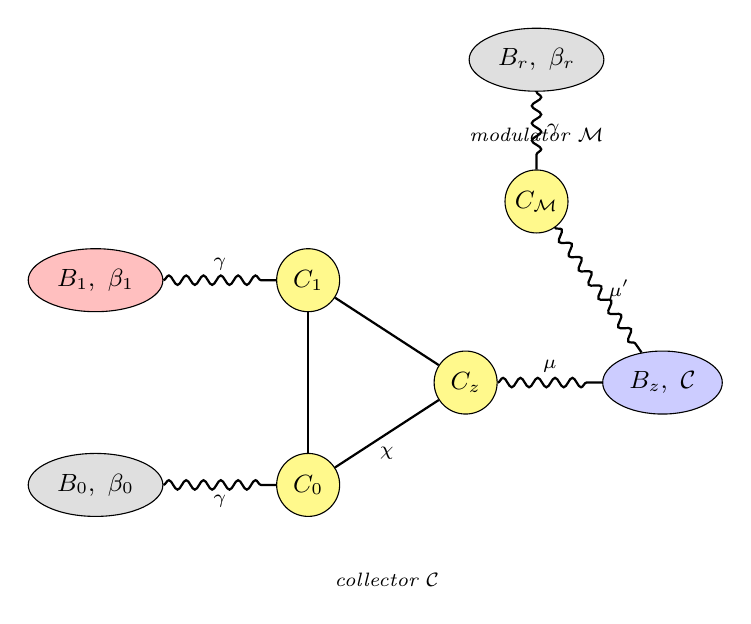
\begin{tikzpicture}[
  qubit/.style={circle, draw, fill=yellow!45, minimum size=8mm,
                inner sep=1pt, font=\small},
  refbath/.style={ellipse, draw, fill=gray!25, minimum width=15mm,
                  minimum height=8mm, font=\small},
  inbath/.style={ellipse, draw, fill=red!25, minimum width=15mm,
                 minimum height=8mm, font=\small},
  outbath/.style={ellipse, draw, fill=blue!20, minimum width=15mm,
                  minimum height=8mm, font=\small},
  therm/.style={decorate, decoration={snake, amplitude=.6mm,
                segment length=2.2mm, post length=1.2mm}, thick},
  coh/.style={thick}
]
% input / reference baths (left)
\node[inbath]  (B1) at (0,1.3)   {$B_1,\ \beta_1$};
\node[refbath] (B0) at (0,-1.3)  {$B_0,\ \beta_0$};
% collector qubits
\node[qubit] (C1) at (2.7,1.3)   {$C_1$};
\node[qubit] (C0) at (2.7,-1.3)  {$C_0$};
\node[qubit] (Cz) at (4.7,0)     {$C_z$};
% finite output reservoir
\node[outbath] (Bz) at (7.2,0)   {$B_z,\ \mathcal{C}$};
% modulator branch
\node[qubit]   (CM) at (5.6,2.3) {$C_\mathcal{M}$};
\node[refbath] (Br) at (5.6,4.1) {$B_r,\ \beta_r$};
% dissipative (thermal) contacts
\draw[therm] (B1) -- (C1) node[midway,above,font=\scriptsize]{$\gamma$};
\draw[therm] (B0) -- (C0) node[midway,below,font=\scriptsize]{$\gamma$};
\draw[therm] (Cz) -- (Bz) node[midway,above,font=\scriptsize]{$\mu$};
\draw[therm] (Br) -- (CM) node[midway,right,font=\scriptsize]{$\gamma$};
\draw[therm] (CM) -- (Bz) node[midway,right,font=\scriptsize]{$\mu'$};
% coherent three-body interaction (drawn as the C0-C1-Cz triangle)
\draw[coh] (C0) -- (C1);
\draw[coh] (C1) -- (Cz);
\draw[coh] (C0) -- (Cz) node[midway,below=1pt,font=\scriptsize]{$\chi$};
% labels for the two modules
\node[font=\scriptsize\itshape] at (3.7,-2.5) {collector $\mathcal{C}$};
\node[font=\scriptsize\itshape] at (5.6,3.15) {modulator $\mathcal{M}$};
\end{tikzpicture}
\caption{Architecture of the original (autonomous) thermodynamic neuron.
Yellow: machine qubits; red: input bath encoding $\beta_1$; grey:
fixed reference baths $\beta_0,\beta_r$; blue: finite output reservoir
$B_z$ (heat capacity $\mathcal{C}$) from which the logical output is
read. Wavy lines are dissipative (thermal) contacts with reset rates
$\gamma,\mu,\mu'$; solid lines depict the single energy--preserving
three--body interaction $H_{\mathrm{int}}$ [Eq.~\eqref{eq:Hint}, drawn as
the $C_0$--$C_1$--$C_z$ triangle], not three independent couplings. The
collector builds the virtual temperature $\beta_v$; the modulator
$C_\mathcal{M}$, straddling $B_r$ and $B_z$, saturates the response.}
\label{fig:Thermodynamic Neuron}
\end{figure}
\subsubsection{The complete Hamiltonian of the machine, term by term}
\label{sec:full-hamiltonian}
The overview above, and the entire population / virtual-temperature
analysis that follows, are consequences of a single microscopic object:
the total Hamiltonian of the machine together with its reservoirs.
Because the rest of Part~1 works with populations and reset-model rates,
it is easy to forget that a Hamiltonian is generating them. This
subsection writes \emph{every} term explicitly, states the Hilbert space
it acts on, and --- most importantly --- justifies why each term has the
form it does and why the terms one might naively expect are deliberately
absent. The reset rates $\gamma,\mu,\mu'$ used from
Sec.~\ref{sec:modulator} onward are nothing but the second-order
(Fermi golden-rule) reductions of the couplings written here; the
population picture is the weak-coupling shadow of this Hamiltonian.

\paragraph{The total Hamiltonian.}
The machine lives on
$\calH = \calH_{S}\otimes\calH_{\mathcal{M}}
\otimes\bigotimes_\alpha \calH_{B_\alpha}$,
where $\calH_S=(\bbC^2)^{\otimes 3}$ carries the three collector qubits
$C_0,C_1,C_z$, $\calH_\mathcal{M}=\bbC^2$ the modulator qubit
$C_\mathcal{M}$, and $\calH_{B_\alpha}$ the reservoirs
$\alpha\in\{0,1,z,r\}$. The generator of the dynamics is
\begin{equation}
H_{\mathrm{tot}}(t)=
\underbrace{H_S+H_{\mathrm{int}}}_{\text{collector}}
\;+\;\underbrace{H_\mathcal{M}}_{\text{modulator}}
\;+\;\underbrace{\sum_\alpha H_{B_\alpha}}_{\text{reservoirs}}
\;+\;\underbrace{\sum_\alpha H_{SB_\alpha}}_{\text{system--bath}}
\;+\;\underbrace{\Delta H_{F}(t)}_{\substack{\text{Floquet extension}\\
(\text{Sec.~\ref{sec:floquet-insertion}})}} .
\label{eq:Htot-machine}
\end{equation}
The last term is zero for the original (autonomous) neuron and is
switched on by the buffer insertion. We take each block in turn.

\paragraph{(1) Free qubit Hamiltonian $H_S$: why two levels, why diagonal.}
\begin{equation}
H_S=\epsilon_0\,n_0+\epsilon_1\,n_1+\epsilon_z\,n_z,
\qquad
n_i:=\ket{1}\!\bra{1}_i=\sigma_+^{(i)}\sigma_-^{(i)}
=\tfrac12\big(\mathbb{1}-\sigma_z^{(i)}\big).
\label{eq:HS}
\end{equation}
\begin{itemize}
\item \emph{Why qubits.} Each node is the two lowest levels of a
physical mode with a well-separated gap $\epsilon_i$; at the
temperatures used, higher levels are thermally inaccessible, so the
truncation to $\{\ket{0},\ket{1}\}$ is controlled.
\item \emph{Why only $\sigma_z$ (no bare transverse field).} The
logical variable is a \emph{population}, i.e.\ a thermal occupation read
in the energy eigenbasis. $H_S$ is therefore chosen diagonal in the
computational basis so that the readout basis is an eigenbasis: a bare
$\sigma_x$ term would rotate the eigenbasis away from the measurement
basis and coherently mix the two logical values. The bare qubits must
be ``idle''---their sole job is to hold populations that the baths and
$H_{\mathrm{int}}$ set.
\item \emph{Why the constants are dropped.} $n_i=\tfrac12(\mathbb1-\sigma_z^{(i)})$
differs from $\tfrac12\sigma_z^{(i)}$ only by an additive constant, which
shifts the zero of energy and never enters any observable.
\item \emph{Resonance conditions (engineered, not automatic).}
We \emph{impose}
$\epsilon_z=\epsilon_0-\epsilon_1$ (so $C_z$ is resonant with the
virtual qubit, below) and $\epsilon_\mathcal{M}=\epsilon_z$ (so the
modulator is resonant with the output channel). These are hardware
design constraints on the fabricated gaps.
\end{itemize}

\paragraph{(2) The collector interaction $H_{\mathrm{int}}$: the term
that does the computation.}
This is the term the population analysis presupposes but never writes.
With the ordering $(C_0C_1C_z)$,
\begin{equation}
\boxed{\;
H_{\mathrm{int}}
= g\big(\ket{100}\!\bra{011}+\ket{011}\!\bra{100}\big)
= g\big(\sigma_+^{(0)}\sigma_-^{(1)}\sigma_-^{(z)}
       +\sigma_-^{(0)}\sigma_+^{(1)}\sigma_+^{(z)}\big).
\;}
\label{eq:Hint}
\end{equation}
Five points justify its form.
\begin{enumerate}[label=(\roman*),leftmargin=*]
\item \textbf{Energy conservation / RWA.} The state $\ket{100}$ has
energy $\epsilon_0$ and $\ket{011}$ has $\epsilon_1+\epsilon_z$; under
the resonance $\epsilon_z=\epsilon_0-\epsilon_1$ these are
\emph{degenerate}. Starting from a generic three-qubit exchange
coupling and passing to the interaction picture, every product of
$\sigma_\pm$'s rotates at a signed sum of the $\epsilon_i$; since
$g\ll\epsilon_i$, all of them average to zero over the free evolution
\emph{except} the resonant pair, which is stationary. That surviving,
secular piece is exactly \eqref{eq:Hint}.
\item \textbf{Why three-body, not pairwise.} The virtual qubit
$\{\ket{01},\ket{10}\}$ is a \emph{joint} property of $C_0$ and $C_1$.
A two-body term $\sigma_+^{(0)}\sigma_-^{(1)}$ would only hop the
excitation between $C_0$ and $C_1$ (an internal rotation of the virtual
qubit) and transfer nothing to $C_z$. Reading the virtual qubit with
$C_z$ therefore requires flipping all three spins at once---an
irreducibly three-body operator.
\item \textbf{The swap interpretation.} In virtual-qubit variables
$\ket{1}_v=\ket{10}$, $\ket{0}_v=\ket{01}$, Eq.~\eqref{eq:Hint} reads
$H_{\mathrm{int}}=g\big(\ket{1}_v\ket{0}_z\bra{0}_v\bra{1}_z
+\mathrm{h.c.}\big)$: a resonant \textsc{swap} (beam splitter) between
the virtual qubit and the target $C_z$. \emph{This is the microscopic
reason $C_z$ equilibrates to the virtual temperature $\beta_v$}---the
interaction literally swaps the virtual qubit's population into $C_z$.
The steady-state population argument of Sec.~\ref{sec:collector-arch}
is the fixed point of this swap.
\item \textbf{Why the non-resonant partners are absent.} Terms such as
$\sigma_+^{(0)}\sigma_+^{(1)}\sigma_+^{(z)}$ create three excitations and
rotate at $\epsilon_0+\epsilon_1+\epsilon_z$; they would inject energy
with no bath to supply it. The RWA discards them with relative error
$\mathcal{O}(g/\epsilon)$.
\item \textbf{Why no bare $C_0$--$C_1$ or $\sigma_z\sigma_z$ coupling.}
The three lines drawn among $C_0,C_1,C_z$ in
Fig.~\ref{fig:buffered-architecture} depict the single three-body term
\eqref{eq:Hint}, \emph{not} three independent pairwise couplings. A
genuine $C_0$--$C_1$ exchange or a dispersive $\sigma_z^{(0)}\sigma_z^{(1)}$
term would hybridise the two input qubits and spoil the product-thermal
structure $\tau_0\otimes\tau_1$ from which the virtual temperature
$\beta_v$ is \emph{defined}; it is deliberately omitted.
\end{enumerate}
\begin{remark}
The resonant pair is $\ket{100}\leftrightarrow\ket{011}$. A tempting but
\emph{wrong} choice is $\ket{101}\leftrightarrow\ket{010}$, which is
detuned by $\epsilon_0+\epsilon_z-\epsilon_1=2\epsilon_z$ and, at
$g\ll\epsilon_z$, is dynamically inert---the collector would not
function. The correct pair is fixed unambiguously by
$\epsilon_0=\epsilon_1+\epsilon_z$.
\end{remark}

\paragraph{(3) Why a bath at all, and the reservoir Hamiltonians.}
Before writing $H_{B_\alpha}$ we answer the conceptual question: why
couple to a bath?
\begin{itemize}
\item \emph{A closed system cannot compute by relaxation.} Unitary
evolution is reversible, has no attractor, and keeps
$S_{vn}[\hat\rho_{\mathrm{tot}}]$ constant; there is no ``settling into
an answer.'' The baths supply the dissipation that drives the machine
to a \emph{unique} nonequilibrium steady state---the logical output.
This is why the effective entropy production
$\Gamma=\partial_t S_{vn}[\hat\rho_s]+\tfrac{1}{\kB}\sum_\alpha
J_\alpha/T_\alpha$ of Sec.~1.1 is nonzero only when the baths are
present.
\item \emph{The baths \textbf{are} the input register.} The logical
input $\beta_1$ \emph{is} a bath temperature; the bias $\beta_0$ is a
bath temperature. There is nowhere else in the model to encode the
inputs.
\item \emph{The temperature gradient is the power supply.} The
autonomous (clockless) gate is driven entirely by heat flowing from hot
to cold reservoirs; with no gradient there is no current and no logic.
\end{itemize}
A bath is thus simultaneously the input register, the power supply, and
the source of irreversibility that makes readout possible---not an
optional add-on. Each reservoir is the standard bosonic (Caldeira--Leggett)
continuum,
\begin{equation}
H_{B_\alpha}=\sum_k \omega_{\alpha k}\,a_{\alpha k}^\dagger a_{\alpha k},
\label{eq:HB}
\end{equation}
a dense harmonic spectrum whose continuum limit yields genuine
irreversible decay (Poincaré recurrence sent to infinity) and whose
Gaussian statistics make it the exact leading-order model of any weakly
coupled environment with the prescribed spectral density. The
system--bath contact is bilinear and \emph{transverse} on the qubit,
\begin{equation}
H_{SB_\alpha}=\sigma_x^{(i(\alpha))}\otimes
\sum_k \lambda_{\alpha k}\big(a_{\alpha k}+a_{\alpha k}^\dagger\big).
\label{eq:HSB}
\end{equation}
\begin{itemize}
\item \emph{Why bilinear.} Leading order in a weak coupling expansion;
higher powers are suppressed and give the Born approximation its
control parameter.
\item \emph{Why $\sigma_x$ and not $\sigma_z$.} To thermalise a qubit
the bath must be able to \emph{flip} it, $\ket{0}\leftrightarrow\ket{1}$,
exchanging the energy quantum $\epsilon_i$;
$\sigma_x=\sigma_++\sigma_-$ does exactly this. A $\sigma_z$ coupling
commutes with $H_i$ and only \emph{dephases}: it could never establish
a thermal population and hence could not encode a temperature. (Contrast
the \emph{drive} of Sec.~\ref{sec:floquet-insertion}, which is chosen
\emph{longitudinal} $\sigma_z$ precisely so that it does \emph{not} pump
populations.)
\item \emph{Detailed balance.} With spectral density
$J_\alpha(\omega)=\pi\sum_k\lambda_{\alpha k}^2\,
\delta(\omega-\omega_{\alpha k})$, the golden-rule rates obey the KMS
condition $\gamma_\alpha(-\omega)=\ee^{-\beta_\alpha\omega}
\gamma_\alpha(\omega)$, which forces qubit $i(\alpha)$ toward the Gibbs
occupation $g\big(\beta_\alpha\epsilon_{i}\big)$. These rates are
precisely the $\gamma,\mu,\mu'$ of the reset model.
\end{itemize}
The bath--to--qubit assignment, and the reason for each, is:
\begin{center}
\begin{tabular}{@{}llll@{}}
\toprule
Bath & Qubit & Inverse temp. & Role \\
\midrule
$B_0$ & $C_0$ & $\beta_0$ (fixed) & reference / perceptron bias \\
$B_1$ & $C_1$ & $\beta_1\in\{\beta_{\mathrm{hot}},\beta_{\mathrm{cold}}\}$
& logical input channel \\
$B_z$ & $C_z$ & $\beta_z(t)$ (\emph{finite}, cap.\ $\mathcal{C}$)
& readout reservoir \\
$B_r$ & $C_\mathcal{M}$ & $\beta_r$ (fixed) & modulator anchor \\
\bottomrule
\end{tabular}
\end{center}
\emph{Why is $B_z$ finite while $B_0,B_1,B_r$ are infinite?} An infinite
reservoir has, by definition, a temperature that does not move---useless
as an output, which must be a variable that \emph{responds} to the
computation. Endowing $B_z$ with a finite heat capacity $\mathcal{C}$
promotes $\beta_z(t)$ to a dynamical calorimetric variable
(Eq.~\eqref{eq:calorimetric}) that integrates the net heat current and
settles at $\beta_z^\infty$: the finiteness of $B_z$ is exactly what
converts a heat \emph{current} into a readable \emph{temperature}.

\paragraph{(4) The modulator Hamiltonian: why one qubit, why two baths.}
\begin{equation}
H_\mathcal{M}=\epsilon_\mathcal{M}\,n_\mathcal{M},
\qquad \epsilon_\mathcal{M}=\epsilon_z,
\end{equation}
in \emph{simultaneous} contact with $B_r$ (rate $\gamma$) and $B_z$
(rate $\mu'$):
\begin{equation}
H_{\mathcal{M}B_r}=\sigma_x^{(\mathcal{M})}\!\otimes\!
\sum_k\lambda_{rk}(a_{rk}+a_{rk}^\dagger),
\qquad
H_{\mathcal{M}B_z}=\sigma_x^{(\mathcal{M})}\!\otimes\!
\sum_k\lambda_{zk}(a_{zk}+a_{zk}^\dagger).
\end{equation}
\begin{itemize}
\item \emph{Why resonant with $C_z$ ($\epsilon_\mathcal{M}=\epsilon_z$).}
The modulator must act on the \emph{same} output channel that the
collector drives, so it competes on equal spectral footing.
\item \emph{Why two baths.} A single-bath qubit merely thermalises to
that bath and does nothing to the output. Straddling the fixed $B_r$ and
the output $B_z$, the modulator becomes a \emph{heat valve} that
continuously pulls $\beta_z$ toward $\beta_r$ (Eq.~\eqref{eq:jM}) with
strength $\mu'$, competing with the collector current. That competition
is what saturates the transfer curve into a sigmoid
(Sec.~\ref{sec:activation}); remove the second bath and the valve---and
with it the whole nonlinearity---disappears, leaving the linear
amplifier flagged in the overview.
\end{itemize}

\paragraph{(5) The Floquet extension $\Delta H_F(t)$: form and
justification.}
For each inserted buffer $F\in\{\mathcal{F}_r,\mathcal{F}_z\}$
(Sec.~\ref{sec:floquet-insertion}), the extension both \emph{adds}
\begin{equation}
\Delta H_F(t)=
\underbrace{\tfrac{\epsilon_F(t)}{2}\,\sigma_z^{(F)}}_{H_F(t),\;
\epsilon_F(t)=\epsilon_F+A\cos\Omega t}
\;+\;\underbrace{g_F\big(\sigma_+^{(C)}\sigma_-^{(F)}+\mathrm{h.c.}\big)}_{H_{CF}}
\;+\;\underbrace{\sigma_x^{(F)}\!\otimes\!\sum_k\lambda_k(a_k+a_k^\dagger)}_{H_{FB}},
\end{equation}
and \emph{moves} the corresponding bath contact off the collector qubit
onto the buffer (the collector reaches $B_0$/$B_z$ only \emph{through}
$F$). Each piece is fixed by a design principle:
\begin{itemize}
\item \emph{Longitudinal drive} ($\propto\sigma_z^{(F)}$, commuting with
$H_F$): it does no work on buffer populations and only dresses the
transition phases, giving the clean Bessel sideband comb
\eqref{eq:jacobi-anger}. A transverse drive $\sigma_x\cos\Omega t$ would
directly pump and heat the buffer and blur the comb.
\item \emph{Resonant exchange $H_{CF}$} (same RWA logic as
$H_{\mathrm{int}}$): transfers excitations between collector qubit and
buffer at no bare-energy cost; counter-rotating $\sigma_x\sigma_x$
pieces are dropped.
\item \emph{Transverse buffer--bath $H_{FB}$} (same reason as
\eqref{eq:HSB}): the buffer must relax through its reservoir.
\item \emph{Only the reference and output branches are dressed.}
Buffering the input branch $C_1$--$B_1$ would alter the logical encoding
\eqref{eq:encoding}; the input is left bare so the bit definition is
untouched.
\end{itemize}

\paragraph{Summary: every term, and what is deliberately absent.}
Table~\ref{tab:hamiltonian-terms} collects the ingredients. The final
row lists the couplings a reader might expect but that are omitted by
design, each for a reason given above.
\begin{table}[h]
\centering\small
\begin{tabularx}{\textwidth}{@{}l l X@{}}
\toprule
\textbf{Term} & \textbf{Expression} &
\textbf{Acts on / role and why this form} \\
\midrule
Free qubits $H_S$ & $\sum_i\epsilon_i n_i$ &
$C_0,C_1,C_z$; holds logical populations. Diagonal only---no transverse
field, so the readout basis is an eigenbasis. \\
Collector $H_{\mathrm{int}}$ & $g(\ket{100}\!\bra{011}+\mathrm{h.c.})$ &
$C_0C_1C_z$; resonant \textsc{swap} of the virtual qubit into $C_z$.
Three-body and secular (RWA); enforces $\epsilon_z=\epsilon_0-\epsilon_1$. \\
Modulator $H_\mathcal{M}$ & $\epsilon_z\,n_\mathcal{M}$ &
$C_\mathcal{M}$; heat-valve anchor, resonant with the output. \\
Reservoirs $H_{B_\alpha}$ & $\sum_k\omega_{\alpha k}a_{\alpha k}^\dagger
a_{\alpha k}$ & $B_{0,1,z,r}$; dissipation, input register, and power
supply. Harmonic continuum. \\
System--bath $H_{SB_\alpha}$ &
$\sigma_x^{(i)}\!\otimes\!\sum_k\lambda_{\alpha k}(a_{\alpha k}
+a_{\alpha k}^\dagger)$ & qubit\,$+$\,bath; thermalises populations.
Transverse ($\sigma_x$) so the bath can flip the qubit; $\sigma_z$ would
only dephase. \\
Buffer drive $H_F(t)$ & $\tfrac{\epsilon_F(t)}{2}\sigma_z^{(F)}$ &
$F$; spectral filter. Longitudinal---no population work. \\
Buffer exchange $H_{CF}$ &
$g_F(\sigma_+^{(C)}\sigma_-^{(F)}+\mathrm{h.c.})$ & $C,F$; mediates
qubit--bath contact. Resonant (RWA). \\
Buffer--bath $H_{FB}$ &
$\sigma_x^{(F)}\!\otimes\!\sum_k\lambda_k(a_k+a_k^\dagger)$ &
$F+$bath; buffer relaxation. Transverse. \\
\midrule
\emph{Absent by design} &
\multicolumn{2}{X@{}}{bare $C_0$--$C_1$ exchange and dispersive
$\sigma_z\sigma_z$ (would spoil $\tau_0\otimes\tau_1$); counter-rotating
three-body terms (non-resonant); transverse bare fields on machine
qubits (would mix logical states); direct collector--bath contact on
dressed branches; a buffer on the input branch (would change the
encoding).} \\
\bottomrule
\end{tabularx}
\caption{Complete term-by-term Hamiltonian of the (Floquet-buffered)
thermodynamic neuron, Eq.~\eqref{eq:Htot-machine}. Each entry names the
support, the physical role, and the design reason for its specific form;
the last row records the couplings that are deliberately excluded.}
\label{tab:hamiltonian-terms}
\end{table}

Everything downstream is a reduction of this Hamiltonian: tracing out
the reservoirs in the weak-coupling, secular limit yields the
reset-model rates $\gamma,\mu,\mu'$ and hence the currents
\eqref{eq:jC}--\eqref{eq:jM}; the population/virtual-temperature
derivation of Sec.~\ref{sec:collector-arch} is the steady state of the
swap \eqref{eq:Hint}; and the buffer terms feed the sideband analysis of
Sec.~\ref{sec:sidebands}. A fully rigorous statement of the reduction,
including the validity window and the induced Lamb shift, is
Proposition~\ref{prop:periodic} in Part~\ref{part:abhishek}.

\subsubsection{The Collector architecture}
\label{sec:collector-arch}
\paragraph{Why need a collector?}
Conisder a classical perceptron model given by :
\[
y = \sum_i\omega_ix_i
\]
before applying an activation function , the perceptron first computes the weigted sum of inputs. So the thermodynamic neuron is analogous to the perceptron model so instead of electrical voltage and the inputs are thermal reservoirs charecterized by their inverse temperature.:
\[
\beta_i =  \frac{1}{K_\beta T_i}
\]
Inside the collector contains 3 qubits \(C_0 , C_1 ,C_z\) where \(C_0 , C_1\) are the input qubits with energy bandgap \(\epsilon_1 , \epsilon_0\) and the \(C_Z\) is the output qubit with band gap \(\epsilon_Z\). \\
Lets first do an numerical rigourous interpretation of the collector:
So there are 2 input qubits \(C_1 \;and \; C_0\) now thses qubits are connected 2 reservoirs \(B_0 , B_1\) amomgst whovht the bath connected to qubit 0 is a constant bath meaning the it acts a refrence , while thebath connected tot qubit 1 is through whoch tht e input is necoded into and sent to the output qubit.The thermal states of each baths are :
\[
\tau_0 = \frac{e^{-\beta_0}}{Z_0} \; , \; \tau_1 = \frac{e^{-\beta_1}}{Z_1}  
\]

For a single qubit the excitation population number is given by :
\[
\mathcal{H}_i = \epsilon_i\ket{1}\bra{1}
\] where the excited propbabailty is 
\[
\mathcal{P}_i(1) = \frac{e^{-\beta_1 \epsilon_i}}{1+\beta_i\epsilon_i} 
\] and the ground state population is given by:
\[
\mathcal{P}_i(0) = \frac{1}{1+\beta_i\epsilon_i}
\] so the boltzman law states that:
\[
\frac{\mathcal{P}(1)} {\mathcal{P}(0) }= e^{-\beta_i \epsilon_1}
\]
Now for the combined system we do the same:
\[
\tau_0
\otimes \tau_1\] Now the basis states are 
\[\ket{00} , \ket{01} , \ket{10} ,\ket{11}\] now the populations for each qubit is :
\[
\mathcal{P}_{00} = p_0(0)p_1(0) \; , \; \\
\mathcal{P}_{01} = p_0(0)p_1(1)\; , \;
\mathcal{P}_{10} = p_0(1)p_1(0)\; , \;
\mathcal{P}_{11} = p_0(1)p_1(1)\; , \;
\]
In the above basis vector state of the system what it is done is that they have defined the states \(\ket{10} , \ket{01}\) as the virtual qubits because unlike the other pure states they form a 2D subspace (the virtual qubit). So mathematically we define \[
\ket{10} = \ket{1}_v \; , \; \ket{01} = \ket{0}_v 
\]
Now calculating the virtual population of the virtual qubits 
\[\mathcal{P}_v(1) = \mathcal{P}_{10} \; , \; \mathcal{P}_v(0) = \mathcal{P}_{01}
\]
Now using the boltzmann ratio we get :
\[
\frac{\mathcal{P}_v(0)}{\mathcal{P}_v(1)}= \frac{\mathcal{P}_0 \mathcal{P}_1}{\mathcal{P}_1 \mathcal{P}_0}
\]
Using the Boltzmann relations

\[
\frac{p_0(0)}{p_0(1)}
=
e^{-\beta_0 \epsilon_0},
\]

and

\[
\frac{p_1(0)}{p_1(1)}
=
e^{-\beta_1 \epsilon_1},
\]

we obtain

\[
\frac{p_1(1)}{p_1(0)}
=
e^{+\beta_1 \epsilon_1}.
\]

Substituting into the population ratio yields

\[
\frac{P_v(0)}{P_v(1)}
=
e^{-\beta_0 \epsilon_0}
e^{+\beta_1 \epsilon_1}.
\]

Hence,

\[
\frac{P_v(0)}{P_v(1)}
=
e^{-(\beta_0\epsilon_0-\beta_1\epsilon_1)}.
\]

Now consider a genuine thermal qubit with energy gap \(E\). Its thermal population ratio is

\[
\frac{P(0)}{P(1)}
=
e^{-\beta E}.
\]

The virtual subspace exhibits exactly the same functional form. We therefore define a virtual energy gap

\[
E_v=\epsilon_0-\epsilon_1,
\]

and a virtual inverse temperature \(\beta_v\) through

\[
\frac{P_v(0)}{P_v(1)}
=
e^{-\beta_v E_v}.
\]

Comparing the exponents gives

\[
\beta_v(\epsilon_0-\epsilon_1)
=
\beta_0\epsilon_0-\beta_1\epsilon_1.
\]

Therefore,

\[
\beta_v
=
\frac{\epsilon_0}{\epsilon_0 -\epsilon_1}\beta_0 - \frac{\epsilon_1}{\epsilon_0 -\epsilon_1}\beta_1
\]

This quantity is called the virtual inverse temperature.

The terminology ``virtual'' is used because no physical thermal reservoir exists at temperature \(T_v=1/(k_B\beta_v)\). Rather, this effective temperature emerges from the population ratio

\[
\frac{P_{01}}{P_{10}}.
\]

The virtual qubit is therefore not a fundamental subsystem but an effective two-level system encoded within the composite Hilbert space of the two thermal qubits \(C_0\) and \(C_1\).

To extract and utilize this virtual temperature, a third qubit \(C_z\) is introduced. Its energy gap is chosen to be resonant with the virtual energy gap:

\[
\epsilon_z
=
\epsilon_0-\epsilon_1
=
E_v.
\]
This \(C_z\) is connected to another bath \(B_z\).so due to this creation of virtual temperature of the initial input quibits the output qubit temperature tries to equalibrize the virtual tenperature or to be more precise the bath connected to the output qubit tries to equilibrate to this virtual temperature resulting in a linear response behaviour making it necessary for the presence of the Modulator.
\subsubsection{Modulator}\label{sec:modulator}
The modulator $\mathcal{M}$ consists of a single qubit $C_\mathcal{M}$ with
energy gap chosen resonant with the output qubit,
\[
\epsilon_\mathcal{M} = \epsilon_z ,
\]
placed in simultaneous contact with \emph{two} baths: the reference bath
$B_r$ at fixed inverse temperature $\beta_r$ (coupling rate $\gamma$) and
the finite output bath $B_z$ (coupling rate $\mu'$). Within the reset
model used for the collector, its state $\rho_\mathcal{M}$ obeys
\begin{equation}
\dot\rho_\mathcal{M}
= \mathcal{L}^{(r)}[\rho_\mathcal{M}] + \mathcal{L}^{(z)}[\rho_\mathcal{M}]
= \gamma\big(\tau(\beta_r)-\rho_\mathcal{M}\big)
+ \mu'\big(\tau(\beta_z)-\rho_\mathcal{M}\big).
\label{eq:mod_ME}
\end{equation}
Since both dissipators are diagonal in the energy basis, it suffices to
track the excited population $p_\mathcal{M} := \bra{1}\rho_\mathcal{M}\ket{1}$:
\begin{equation}
\dot p_\mathcal{M}
= \gamma\big[g(\beta_r\epsilon_z)-p_\mathcal{M}\big]
+ \mu'\big[g(\beta_z\epsilon_z)-p_\mathcal{M}\big].
\end{equation}
Setting $\dot p_\mathcal{M}=0$ gives the exact steady-state population
\begin{equation}
p_\mathcal{M}^{\,ss}
= \frac{\gamma\, g_z(\beta_r) + \mu'\, g_z(\beta_z)}{\gamma+\mu'}
\;\xrightarrow{\;\mu'\ll\gamma\;}\; g_z(\beta_r),
\label{eq:mod_ss}
\end{equation}
i.e.\ in the regime $\mu'\ll\gamma$ the modulator qubit is pinned to the
reference temperature $\beta_r$, essentially unperturbed by the output
bath. The heat current it delivers to $B_z$ under the reset model is then
\begin{equation}
j_\mathcal{M} = \mu'\,\epsilon_z\big[g_z(\beta_z)-g_z(\beta_r)\big].
\label{eq:jM}
\end{equation}
The modulator therefore continuously pulls $\beta_z$ toward $\beta_r$
with strength $\mu'$. This is the entire mechanism: it is a
\emph{single-qubit heat valve} between $B_r$ and $B_z$ that competes
with the collector current. The two free parameters $(\beta_r,\mu')$
will be fixed below so that the competition confines $\beta_z^\infty$ to
a designated logical window, which is precisely what converts the linear
amplifier of Sec.~\ref{sec:collector-arch} into a saturating,
sigmoid-like response.
 
\subsubsection{Dynamics of the full machine: two time scales}
\label{sec:dynamics}
Collecting the two currents into $B_z$ --- the collector current
\begin{equation}
j_\mathcal{C} = \mu\,\epsilon_z\big[g_z(\beta_z)-g_z(\beta_v)\big],
\label{eq:jC}
\end{equation}
derived in Sec.~\ref{sec:collector-arch} from the virtual-qubit
resonance, and the modulator current \eqref{eq:jM} --- the finite bath
$B_z$ with heat capacity $\mathcal{C}$ evolves according to the
calorimetric equation $\dot T_z = (j_\mathcal{C}+j_\mathcal{M})/\mathcal{C}$,
which in terms of $\beta_z = 1/(\kB T_z)$ reads
\begin{equation}
\dot\beta_z
= -\frac{\kB\beta_z^{2}}{\mathcal{C}}\,\big(j_\mathcal{C}+j_\mathcal{M}\big).
\label{eq:calorimetric}
\end{equation}
The consistency of using the \emph{steady-state} expressions
\eqref{eq:jC} and \eqref{eq:jM} inside \eqref{eq:calorimetric} rests on
a separation of time scales enforced by construction,
\begin{equation}
\gamma \;\gg\; \mu,\;\mu' ,
\end{equation}
so that the internal (fast) relaxation of $\mathcal{C}$ and $\mathcal{M}$
is slaved to the instantaneous value of $\beta_z(t)$: on the fast scale
$C_z$ thermalizes to $\beta_v$ and $C_\mathcal{M}$ to $\beta_r$, while on
the slow scale $\beta_z(t)$ drifts under the residual currents. This is
an adiabatic elimination of the machine's internal degrees of freedom
and is the autonomous analogue of the quasi-static gate assumption in
CMOS analysis.
 
\subsubsection{Steady state and the activation function}
\label{sec:activation}
The nonequilibrium steady state of the output is defined by
$\dot\beta_z=0$, i.e.\ $j_\mathcal{C}+j_\mathcal{M}=0$. Substituting
\eqref{eq:jC} and \eqref{eq:jM},
\begin{equation}
(\mu+\mu')\,g_z(\beta_z^\infty)
= \mu\, g_z(\beta_v) + \mu'\, g_z(\beta_r),
\end{equation}
hence, defining the branching ratio $\Delta := \mu/(\mu+\mu')$,
\begin{equation}
\boxed{\;
g_z(\beta_z^\infty)
= \Delta\, g_z(\beta_v) + (1-\Delta)\, g_z(\beta_r)
\;}
\label{eq:ss_condition}
\end{equation}
The steady-state excitation of the output channel is a convex
combination of the collector's target ($\beta_v$) and the modulator's
anchor ($\beta_r$), weighted purely by coupling rates. Inverting
$g_z(\beta) = (1+\ee^{\beta\epsilon_z})^{-1}$,
\begin{equation}
\beta_z^\infty
= \frac{1}{\epsilon_z}\,
\ln\!\left[\frac{1}{\Delta\, g_z(\beta_v)+(1-\Delta)\,g_z(\beta_r)}-1\right].
\label{eq:betainf_general}
\end{equation}
 
\paragraph{Fixing the modulator: confinement to the logical window.}
For $\beta_z^\infty$ to serve as a logical signal we demand that it be
confined to a window $[\beta_{\mathrm{hot}},\beta_{\mathrm{cold}}]$
(with $\beta_{\mathrm{cold}}>\beta_{\mathrm{hot}}$) even when the
virtual temperature saturates. Since $g_z$ is monotonically decreasing,
$\beta_v\to+\infty$ gives $g_z(\beta_v)\to 0$ and
$\beta_v\to-\infty$ gives $g_z(\beta_v)\to 1$. Imposing
\begin{align}
\beta_v\to +\infty &: \quad
(1-\Delta)\,g_z(\beta_r) \overset{!}{=} g_z(\beta_{\mathrm{cold}}),
\label{eq:constraint1}\\
\beta_v\to -\infty &: \quad
\Delta + (1-\Delta)\,g_z(\beta_r) \overset{!}{=} g_z(\beta_{\mathrm{hot}}),
\label{eq:constraint2}
\end{align}
and subtracting \eqref{eq:constraint1} from \eqref{eq:constraint2},
\begin{equation}
\Delta = g_z(\beta_{\mathrm{hot}}) - g_z(\beta_{\mathrm{cold}}),
\qquad
g_z(\beta_r) = \frac{g_z(\beta_{\mathrm{cold}})}{1-\Delta}.
\label{eq:mod_design}
\end{equation}
These two design equations fix $(\mu'/\mu,\beta_r)$ in terms of the
chosen logical window. Substituting back into
\eqref{eq:betainf_general},
\begin{equation}
\beta_z^\infty = \frac{1}{\epsilon_z}\ln\!\big[Q(\beta_v)^{-1}-1\big],
\qquad
Q(\beta_v) := g_z(\beta_{\mathrm{hot}})\,g_z(\beta_v)
+ g_z(\beta_{\mathrm{cold}})\big(1-g_z(\beta_v)\big).
\label{eq:transfer}
\end{equation}
Equation \eqref{eq:transfer} is the exact transfer characteristic of
the neuron under the reset model.
 
\paragraph{Emergence of the sigmoid.}
The connection to the perceptron activation is transparent once one
notices an \emph{exact} identity. From the definition of the virtual
temperature, $\beta_v\epsilon_z = \beta_0\epsilon_0-\beta_1\epsilon_1$,
so with $f(x):=(1+\ee^{x})^{-1}$,
\begin{equation}
g_z(\beta_v)
= \frac{1}{1+\ee^{\beta_v\epsilon_z}}
= f\big(\beta_0\epsilon_0-\beta_1\epsilon_1\big)
\qquad \text{(no approximation)} .
\label{eq:exact_sigmoid}
\end{equation}
The sigmoid is thus already present at the level of the virtual-qubit
population; the modulator's role is to map it affinely onto the
temperature axis. Indeed, expanding \eqref{eq:transfer} for small
$\epsilon_z$ (with $\beta_{\mathrm{hot}},\beta_{\mathrm{cold}}$ of order
unity): using $g_z(\beta)=\tfrac12-\tfrac{\beta\epsilon_z}{4}
+\mathcal{O}(\epsilon_z^{3})$,
\begin{align}
Q(\beta_v)
&= \tfrac12 - \frac{\epsilon_z}{4}
\Big[\beta_{\mathrm{cold}}
- (\beta_{\mathrm{cold}}-\beta_{\mathrm{hot}})\,g_z(\beta_v)\Big]
+\mathcal{O}(\epsilon_z^{2}) ,\\[2pt]
\beta_z^\infty
&= \frac{1}{\epsilon_z}
\ln\frac{1-Q}{Q}
= \frac{1}{\epsilon_z}
\ln\!\left[1+\epsilon_z
\Big(\beta_{\mathrm{cold}}
-(\beta_{\mathrm{cold}}-\beta_{\mathrm{hot}})\,g_z(\beta_v)\Big)
+\mathcal{O}(\epsilon_z^{2})\right] \nonumber\\[2pt]
&= \beta_{\mathrm{hot}}\, g_z(\beta_v)
+ \beta_{\mathrm{cold}}\big(1-g_z(\beta_v)\big)
+ \mathcal{O}(\epsilon_z).
\label{eq:activation}
\end{align}
Equations \eqref{eq:exact_sigmoid}--\eqref{eq:activation} together give
\begin{equation}
\beta_z^\infty
\simeq \beta_{\mathrm{cold}}
+ (\beta_{\mathrm{hot}}-\beta_{\mathrm{cold}})\,
f\big(\epsilon_0(\beta_0-\beta_1) + \beta_1\epsilon_z\big),
\end{equation}
a sigmoidal interpolation between the two logical rails whose argument
is the perceptron pre-activation: weight $\epsilon_1$
(steepness $\propto\epsilon_0\approx\epsilon_1$ for small
$\epsilon_z$), bias set by $\beta_0$. In the limit
$\epsilon_1\to\infty$ the transfer characteristic approaches the ideal
inverted step function; the price, as quantified by the entropy
production analysis of \cite{LipkaBartosik2024}, is monotonically
increasing dissipation --- the error--dissipation tradeoff that
Part~\ref{part:abhishek}, Conjecture~\ref{conj:tradeoff}, generalizes to
the driven setting.
 
\subsubsection{Logic encoding and the NOT operation}
\label{sec:logic}
Logical values are encoded and decoded via
\begin{equation}
x = \begin{cases}
0, & \beta_1 = \beta_{\mathrm{hot}},\\
1, & \beta_1 = \beta_{\mathrm{cold}},
\end{cases}
\qquad
y = \begin{cases}
0, & \beta_z^{\infty} \le (1+\delta)\,\beta_{\mathrm{hot}},\\
1, & \beta_z^{\infty} \ge (1-\delta)\,\beta_{\mathrm{cold}},\\
\varnothing & \text{otherwise},
\end{cases}
\label{eq:encoding}
\end{equation}
where $\delta$ is a tolerance defining guard bands around the rails and
$\varnothing$ marks an invalid readout. The inversion follows directly
from the sign structure of $\beta_v$: for a hot input
($\beta_1=\beta_{\mathrm{hot}}<\beta_0$) the collector operates as a
refrigerator, $\beta_v$ is large, $g_z(\beta_v)\to 0$, and
\eqref{eq:activation} gives $\beta_z^\infty\to\beta_{\mathrm{cold}}$
($y=1$); for a cold input the collector is a heat pump,
$g_z(\beta_v)\to 1$, and $\beta_z^\infty\to\beta_{\mathrm{hot}}$
($y=0$). Fluctuations of the finite bath around $\beta_z^\infty$
(Gaussian with width controlled by $\mathcal{C}$) produce a nonzero
error probability $\langle\xi\rangle$; it is exactly this readout
fragility --- logical information carried by a fluctuating classical
temperature at the end of an open, bidirectional channel --- that
motivates the buffer architecture of the next subsection.
 
% =====================================================================
\subsection{Insertion of the Floquet buffers}
\label{sec:floquet-insertion}
We now make the proposal of Sec.~1.2 concrete. Two buffers are
inserted:
\begin{itemize}
\item $\mathcal{F}_r$ in the \emph{reference branch}, mediating
$C_0 \leftrightarrow \mathcal{F}_r \leftrightarrow B_0$;
\item $\mathcal{F}_z$ in the \emph{output branch}, mediating
$C_z \leftrightarrow \mathcal{F}_z \leftrightarrow B_z$.
\end{itemize}
The input branch $C_1\!-\!B_1$ is left undressed so that the logical
encoding is untouched. Each buffer is a two-level system with a
periodically modulated gap,
\begin{equation}
H_{\mathcal{F}}(t)
= \frac{\epsilon_F(t)}{2}\,\sigma_z^{(F)},
\qquad
\epsilon_F(t) = \epsilon_F + A\cos(\Omega t),
\qquad
H_\mathcal{F}(t+T)=H_\mathcal{F}(t),\;\; T = \frac{2\pi}{\Omega},
\label{eq:bufferH}
\end{equation}
coupled (i) to its neighbouring collector qubit by a resonant
excitation-exchange term of strength $g_F$,
$H_{CF} = g_F(\sigma_+^{(C)}\sigma_-^{(F)} + \mathrm{h.c.})$, and
(ii) to its bath by a standard bilinear coupling
$H_{FB} = \sigma_x^{(F)}\otimes \sum_k \lambda_k (a_k + a_k^\dagger)$
with spectral density $J(\omega)$ and KMS-obeying rates
$\gamma(\omega)$, i.e.\ $\gamma(-\omega)=\ee^{-\beta\omega}\gamma(\omega)$.
The modulated-gap (longitudinal) drive is chosen deliberately: it
commutes with $\sigma_z^{(F)}$, so the drive does no work on the buffer
populations directly; it only dresses the \emph{phases} of the
transition operators, which is exactly the handle needed for spectral
filtering.
 
\subsubsection{Sideband decomposition of the buffer--bath coupling}
\label{sec:sidebands}
In the interaction picture with respect to $H_\mathcal{F}(t)$, the
lowering operator of the buffer accumulates the integrated phase
\begin{equation}
\sigma_-^{(F)}(t)
= \sigma_-^{(F)}\,
\exp\!\Big[-\ii\!\int_0^t \epsilon_F(t')\,\d t'\Big]
= \sigma_-^{(F)}\,
\ee^{-\ii\epsilon_F t}\,
\ee^{-\ii \frac{A}{\Omega}\sin(\Omega t)} .
\end{equation}
The Jacobi--Anger expansion
$\ee^{-\ii z\sin\theta} = \sum_{q\in\bbZ} J_q(z)\,\ee^{-\ii q\theta}$
(with $J_q$ the Bessel function of the first kind) resolves this into a
sideband comb:
\begin{equation}
\boxed{\;
\sigma_-^{(F)}(t)
= \sigma_-^{(F)} \sum_{q\in\bbZ}
J_q\!\Big(\tfrac{A}{\Omega}\Big)\,
\ee^{-\ii(\epsilon_F + q\Omega)t}
\;}
\label{eq:jacobi-anger}
\end{equation}
The single transition line at $\epsilon_F$ is replaced by lines at
$\epsilon_F+q\Omega$ with weights $J_q^2(A/\Omega)$ --- this is the
quantum-optical content of the FM analogy of
Sec.~\ref{sec:floquet-examples}: the modulation index $\beta_{\rm FM}$
of the communication example is literally $A/\Omega$ here, and the
Carson bandwidth of FM corresponds to the width of the populated
sideband comb. Inserting \eqref{eq:jacobi-anger} into the second-order
(Floquet--Born--Markov) golden-rule rates and applying the secular
approximation with respect to the drive (valid for
$\Omega \gg \gamma(\epsilon_F)$, so cross-sideband interference terms
average out), the downward and upward rates on the buffer become
\begin{align}
\Gamma_\downarrow
&= \sum_{q} J_q^2\!\Big(\tfrac{A}{\Omega}\Big)\,
\gamma\big(\epsilon_F + q\Omega\big),
\label{eq:Gdown}\\
\Gamma_\uparrow
&= \sum_{q} J_q^2\!\Big(\tfrac{A}{\Omega}\Big)\,
\gamma\big(-\epsilon_F - q\Omega\big)
= \sum_{q} J_q^2\!\Big(\tfrac{A}{\Omega}\Big)\,
\ee^{-\beta(\epsilon_F+q\Omega)}\,
\gamma\big(\epsilon_F + q\Omega\big),
\label{eq:Gup}
\end{align}
where the last equality used the KMS condition of the physical bath at
inverse temperature $\beta$. Equations
\eqref{eq:Gdown}--\eqref{eq:Gup} are the Tien--Gordon structure of
photon-assisted transport \cite{TienGordon1963,Grifoni1998}: the driven
buffer samples the bath spectral function at a comb of frequencies,
with Bessel weights controlled by the single dimensionless knob
$A/\Omega$.
 
Two filtering mechanisms follow immediately.
\emph{(i) Line suppression:} at the zeros of $J_0$
($A/\Omega \approx 2.405, 5.520,\dots$) the carrier transition at
$\epsilon_F$ is dynamically switched off --- coherent destruction of
the direct thermal channel --- while sidebands remain open. \emph{(ii)
Spectral relocation:} by choosing $\Omega$ so that
$\epsilon_F + q^\ast\Omega$ sits where $J(\omega)$ is large (or in a
gap), a single sideband $q^\ast$ can be made to dominate the sums.
 
\subsubsection{Floquet-synthesized effective temperature}
\label{sec:eff-temp}
The driven buffer does not merely rescale the coupling; it changes the
\emph{detailed-balance ratio} seen at the buffer gap. Define the
effective inverse temperature $\beta_{\mathrm{eff}}$ of the dressed
environment by
\begin{equation}
\ee^{-\beta_{\mathrm{eff}}\,\epsilon_F}
:= \frac{\Gamma_\uparrow}{\Gamma_\downarrow}
= \frac{\sum_q J_q^2(A/\Omega)\,
\ee^{-\beta(\epsilon_F+q\Omega)}\,\gamma(\epsilon_F+q\Omega)}
{\sum_q J_q^2(A/\Omega)\,\gamma(\epsilon_F+q\Omega)} .
\label{eq:beta_eff}
\end{equation}
For $A=0$ only $q=0$ survives and $\beta_{\mathrm{eff}}=\beta$, as it
must. In the single-sideband regime where $q^\ast$ dominates,
\begin{equation}
\beta_{\mathrm{eff}}
\approx \beta\,\frac{\epsilon_F+q^\ast\Omega}{\epsilon_F},
\label{eq:beta_eff_single}
\end{equation}
so the same physical bath at $\beta$ is presented to the collector as
an effective bath that is colder ($q^\ast>0$), hotter
($-\epsilon_F<q^\ast\Omega<0$), or even population-inverted
($q^\ast\Omega<-\epsilon_F$, $\beta_{\mathrm{eff}}<0$). In general
\eqref{eq:beta_eff} is not of Gibbs form across different gaps --- the
dressed environment is athermal --- but on the single relevant
transition of $C_0$ (which exchanges excitations resonantly with
$\mathcal{F}_r$ at rate $g_F$, and is therefore slaved to the buffer's
steady population in the regime
$g_F \gg \Gamma_\downarrow+\Gamma_\uparrow \gg \mu$) it acts exactly as
a thermal reservoir at $\beta_{\mathrm{eff}}$. A rigorous derivation of
this statement, including the conditions under which the composite
$\mathcal{F}\!+\!B$ admits Markovian elimination and the form of the
induced Lamb shift, is the content of
Proposition~\ref{prop:periodic} in Part~\ref{part:abhishek}; here we
take the physical picture and draw its consequences for the neuron.
 
\subsubsection{Consequence I: drive-tunable weights and bias}
\label{sec:tunable-weights}
Replacing $\beta_0 \to \beta_{\mathrm{eff}}(A/\Omega,\Omega)$ in the
virtual temperature,
\begin{equation}
\beta_v^{\mathrm{eff}}
= \frac{\epsilon_0}{\epsilon_0-\epsilon_1}\,
\beta_{\mathrm{eff}}\!\Big(\tfrac{A}{\Omega},\Omega\Big)
- \frac{\epsilon_1}{\epsilon_0-\epsilon_1}\,\beta_1 ,
\label{eq:betav_eff}
\end{equation}
the reference-branch buffer promotes the perceptron \emph{bias} from a
hardware constant to a runtime control parameter. In the autonomous
neuron the weights and bias are frozen into the fabricated energy gaps
$\epsilon_i$ and the physical reference temperature $\beta_0$; training
or reconfiguring the gate means re-engineering the hardware. With
$\mathcal{F}_r$ in place, the threshold location of the activation
\eqref{eq:activation} --- which sits at
$\beta_1 \approx \beta_{\mathrm{eff}}$ for small $\epsilon_z$ --- is
swept electrically/optically through $A/\Omega$ without touching any
qubit gap. The same neuron can thus be repurposed (e.g.\ shifting the
NOT threshold, or, in the multi-input generalization, retraining a
linearly separable function \emph{in situ}) at the cost of drive work.
This is, to our knowledge, the feature that most sharply distinguishes
the buffered architecture from the autonomous one: it trades autonomy
for programmability, in direct analogy with the gate terminal of a
transistor.
 
\subsubsection{Consequence II: output-branch buffer as a gated,
rectifying readout stage}
\label{sec:output-buffer}
The output buffer $\mathcal{F}_z$ addresses the readout fragility
identified in Sec.~\ref{sec:logic}. Two mechanisms operate.
 
\paragraph{(a) Spectral rectification (suppressing backflow).}
The current from $B_z$ back into the collector is carried by the same
comb \eqref{eq:Gdown}--\eqref{eq:Gup}. Because absorption and emission
sample $\gamma(\pm(\epsilon_F+q\Omega))$ asymmetrically whenever the
comb straddles regions where $J(\omega)$ varies strongly, the ratio of
forward (collector$\to B_z$) to backward conductance can be engineered
away from unity. Operating $\mathcal{F}_z$ near a $J_0$ zero with a
single dominant blue sideband placed at a peak of $J(\omega)$ makes the
effective channel predominantly emissive into $B_z$: the buffer behaves
as an energy diode for the readout current. Within the effective-rate
description, this replaces the symmetric reset coupling $\mu$ of
Eq.~\eqref{eq:jC} by an asymmetric pair
$(\mu_\rightarrow, \mu_\leftarrow)$ with
$\mu_\leftarrow/\mu_\rightarrow < 1$, which steepens the approach of
$\beta_z(t)$ to its fixed point and reduces the sensitivity of
$\beta_z^\infty$ to fluctuations of the finite bath --- i.e.\ it widens
the usable guard band $\delta$ in \eqref{eq:encoding} at fixed error
rate.
 
\paragraph{(b) Stroboscopic gating.}
Since the comb weights depend on $A/\Omega$, ramping $A$ between
$A_{\rm on}$ and a $J_0$ zero periodically opens and closes the
$C_z\!-\!B_z$ channel in synchrony with an external clock. The neuron
then integrates its computation while the channel is shut (no
information leaks to, and no noise enters from, $B_z$) and commits the
result during short readout windows. This is precisely the
clock-gateway mechanism that Ref.~\cite{LipkaBartosik2024} introduces
externally to concatenate neurons into networks (their
Supplementary Material~C), here realized \emph{inside} the machine by
the drive itself: $t_{\rm steady}$ and $t_{\rm const}$ of their
protocol map onto the closed and open fractions of the drive period.
The buffered neuron is therefore natively composable, at the price of
no longer being autonomous.
 
\subsubsection{Cost accounting and outlook of Part 1}
\label{sec:cost}
Both consequences are paid for in work. The drive injects average power
$P_{\rm drive}(t) = \expect{\partial_t H_\mathcal{F}(t)}$, and every
sideband-assisted exchange of a bath quantum $\epsilon_F+q\Omega$
transfers $q\Omega$ from the drive per event; the effective-temperature
shift \eqref{eq:beta_eff_single} is thus a work-powered refrigeration
or pumping effect, consistent with the second law for periodically
driven open systems \cite{Brandner2016}. Whether the gain in logical
distinguishability can outrun this cost --- and what the optimal
exchange rate is --- is exactly the work--distinguishability tradeoff
formalized as Conjecture~\ref{conj:tradeoff} and probed numerically in
the staged programme of Part~\ref{part:abhishek},
Sec.~\ref{sec:numerics}. The weak-coupling regime in which the
effective-rate picture of this section is quantitatively valid is
delimited by Proposition~\ref{prop:periodic}; the non-Markovian regime,
where the buffer correlation time competes with $1/g_F$ and the
sideband picture breaks down, requires the chain-mapped MPS machinery
of Sec.~\ref{sec:nonMarkovian}.
\subsection{Validity window, breakdown, and numerical stability}
\label{sec:validity}
 
\subsubsection{Hierarchy of scales and the validity window}
\label{sec:hierarchy}
The effective-rate picture of Secs.~\ref{sec:sidebands}--\ref{sec:eff-temp}
is a chain of three eliminations, each with its own small parameter.
Denote by
\begin{equation}
\Gamma_F := \Gamma_\downarrow + \Gamma_\uparrow
= \sum_q J_q^2\!\Big(\tfrac{A}{\Omega}\Big)
\Big[1+\ee^{-\beta(\epsilon_F+q\Omega)}\Big]\,
\gamma(\epsilon_F+q\Omega)
\label{eq:GammaF}
\end{equation}
the total dressed linewidth of the buffer, i.e.\ the inverse of its
correlation time $\tau_c = 1/\Gamma_F$ in the periodic steady state.
The three approximations and their control parameters are:
\begin{enumerate}[label=(V\arabic*),leftmargin=*]
\item \textbf{Drive-secular approximation.} Cross-sideband
interference terms in the dissipator oscillate at multiples of
$\Omega$ and average out over the buffer relaxation time provided
\begin{equation}
\eta_1 := \frac{\Gamma_F}{\Omega} \ll 1 .
\end{equation}
When $\eta_1\sim 1$ the sidebands overlap within their linewidth: the
comb \eqref{eq:jacobi-anger} merges into a continuum and the weights
$J_q^2$ lose meaning individually.
\item \textbf{Born--Markov elimination of the buffer.} Treating the
buffer$+$bath compound as a Markovian environment for $C_0$ requires
its correlation time to be short compared to the induced relaxation of
$C_0$. The induced rate is of order $g_F^2/\Gamma_F$
(second-order golden rule against a Lorentzian of width $\Gamma_F$), so
Markovianity requires
\begin{equation}
\eta_2 := \frac{g_F}{\Gamma_F} \ll 1 ,
\qquad
\text{relative error of the Lindblad reduction} = \mathcal{O}(\eta_2^{2}).
\label{eq:markov-error}
\end{equation}
The error estimate follows from the Nakajima--Zwanzig expansion: the
first neglected (fourth-order) contribution to the memory kernel is
suppressed relative to the second-order one by
$(g_F\tau_c)^2 = \eta_2^2$.
\item \textbf{Slaving of the slow calorimetric variable.} The dressed
channel into $B_z$ must remain the slowest process,
\begin{equation}
\eta_3 := \frac{\mu_{\mathrm{eff}}}{g_F^2/\Gamma_F} \ll 1,
\qquad
\mu_{\mathrm{eff}} := \text{effective } C_z\!-\!B_z \text{ rate through } \mathcal{F}_z .
\end{equation}
\end{enumerate}
The window in which every result of
Secs.~\ref{sec:sidebands}--\ref{sec:output-buffer} is quantitatively
controlled is therefore the nested hierarchy
\begin{equation}
\boxed{\;
\mu_{\mathrm{eff}} \;\ll\; \frac{g_F^{2}}{\Gamma_F}
\;\ll\; \Gamma_F \;\ll\; \Omega \;\lesssim\; \epsilon_F
\;}
\label{eq:hierarchy}
\end{equation}
with cumulative error
$\mathcal{O}(\eta_1)+\mathcal{O}(\eta_2^2)+\mathcal{O}(\eta_3)$.
Note the structural tension already flagged in
Proposition~\ref{prop:periodic}: making the buffer--bath coupling
weaker (to protect the buffer's periodic steady state) \emph{lengthens}
$\tau_c$ and therefore shrinks the admissible $g_F$ through
\eqref{eq:markov-error}. The window \eqref{eq:hierarchy} is real but
narrow; everything outside it belongs to the non-Markovian programme.
 
\subsubsection{The buffer as a tunable filtered environment}
\label{sec:Jeff}
The physical content of the elimination (V2) is an effective spectral
density. Linearizing the buffer around low excitation
($\sigma_-^{(F)}\!\to b$, valid for
$\Gamma_\uparrow/\Gamma_F \ll 1$, i.e.\ an effectively cold dressed
buffer; for larger thermal occupancy the qubit nonlinearity adds a
saturation correction of order $\Gamma_\uparrow/\Gamma_F$), the
buffer is a damped mode and the compound
$\mathcal{F}\!+\!B$ presents to $C_0$ the Lorentzian-comb spectral
density
\begin{equation}
J_{\mathrm{eff}}(\omega)
= \frac{g_F^{2}}{\pi}
\sum_{q\in\bbZ} J_q^{2}\!\Big(\tfrac{A}{\Omega}\Big)\,
\frac{\Gamma_F/2}{\big(\omega-\epsilon_F-q\Omega\big)^{2}
+ \big(\Gamma_F/2\big)^{2}} .
\label{eq:Jeff}
\end{equation}
Equation \eqref{eq:Jeff} makes the ``spectral and temporal filter''
statement of Sec.~1.2 quantitative: the drive relocates the weight of
the comb ($q$, controlled by $\Omega$), reweights it ($J_q^2$,
controlled by $A/\Omega$), and the buffer--bath coupling sets the
tooth width $\Gamma_F$. Markovianity of the reduced $C_0$ dynamics is
the statement that $J_{\mathrm{eff}}$ is flat across the linewidth
$g_F^2/\Gamma_F$ of the qubit --- automatically satisfied inside
\eqref{eq:hierarchy} because linewidth/toothwidth $=\eta_2^2$.
 
The corresponding memory kernel of the Nakajima--Zwanzig equation for
$C_0$,
\begin{equation}
K(\tau) \;\propto\; g_F^{2}\,
\ee^{-\Gamma_F\tau/2}
\sum_q J_q^{2}\!\Big(\tfrac{A}{\Omega}\Big)
\cos\!\big[(\epsilon_F+q\Omega)\tau\big],
\qquad \tau\ge 0,
\label{eq:kernel}
\end{equation}
decays exponentially with rate $\Gamma_F/2$ --- Assumption (A2) of
Part~\ref{part:abhishek} holds with
$\tau_c = 2/\Gamma_F$. \textbf{Breakdown} occurs when
$g_F\gtrsim\Gamma_F$: the poles of the $C_0$--buffer propagator split
by $\pm g_F$ (vacuum-Rabi doublet), $K(\tau)$ acquires undamped
oscillations at $g_F$, the time-convolutionless expansion ceases to
converge, and information flows back from the buffer into $C_0$ within
a drive period. A convenient numerical diagnostic is the BLP
trace-distance witness: propagate two initial states
$\rho_{1,2}(0)$ of $C_0$ and monitor
\begin{equation}
\sigma(t) := \dv{t}\, D\big(\rho_1(t),\rho_2(t)\big);
\qquad
\sigma(t) > 0 \;\Rightarrow\; \text{information backflow}
\;\Rightarrow\; \text{sideband picture invalid at } t .
\label{eq:BLP}
\end{equation}
$\sigma(t)>0$ episodes are exactly the entropy-production
back\-flow pathology described in Sec.~1.1, now with a measurable
marker; the buffered design succeeds precisely to the extent that the
drive parameters can push $\max_t\sigma(t)\to 0^+$ on the collector
while retaining gain.
 
\subsubsection{Numerical stability of the multiscale problem}
\label{sec:numstab}
The buffered neuron is numerically stiff by construction: the rate
spectrum spans
$\mu_{\mathrm{eff}}\sim 10^{-4} \ll \gamma,\chi \sim 1 \ll
\Omega \sim 10$--$10^{2}$ (in units of $\epsilon_z^{-1}$ taken as 1),
a stiffness ratio $\kappa = \Omega/\mu_{\mathrm{eff}}\gtrsim 10^{5}$.
A naive explicit integration of the full master equation must resolve
$h \lesssim 2\pi/(10\,\Omega)$ over a horizon
$t_{\mathrm{slow}}\sim \mathcal{C}/\mu_{\mathrm{eff}}$, i.e.\
$\gtrsim 10^{7}$--$10^{9}$ steps with error accumulation that destroys
the small currents $j_\mathcal{C}+j_\mathcal{M}\to 0$ near the fixed
point. The stable scheme mirrors the physics
(Sec.~\ref{sec:dynamics}): exploit the same time-scale separation the
machine itself uses.
 
\paragraph{Two-tier integrator.}
\begin{enumerate}[leftmargin=*]
\item \textbf{Fast tier (per grid point).} Freeze $\beta_z$. Solve the
Floquet--Lindblad equation for the machine qubits over one period $T$
to its periodic steady state (QuTiP: \texttt{FloquetBasis} /
\texttt{fmmesolve}; or evolve $\ee^{\mathcal{L}_{\mathrm{eff}}T}$ and
take its Perron eigenvector). Extract the period-averaged currents
$\bar\jmath_\mathcal{C}(\beta_z)$, $\bar\jmath_\mathcal{M}(\beta_z)$,
$\bar P_{\mathrm{drive}}(\beta_z)$.
\item \textbf{Slow tier.} Integrate the scalar ODE
\begin{equation}
\dot\beta_z = -\frac{\kB\beta_z^{2}}{\mathcal{C}}
\big[\bar\jmath_\mathcal{C}(\beta_z)+\bar\jmath_\mathcal{M}(\beta_z)\big]
\label{eq:slowODE}
\end{equation}
with any $\mathcal{O}(h^4)$ nonstiff method, interpolating
$\bar\jmath(\beta_z)$ from a precomputed grid ($\sim$30--50 points
suffice; the currents are smooth, monotone functions of
$g_z(\beta_z)$ by \eqref{eq:jC},\eqref{eq:jM}).
\end{enumerate}
The scheme replaces $10^{8}$ coupled steps by
$\mathcal{O}(10^{2})$ fast-tier solves; its systematic error is the
adiabatic-elimination error $\mathcal{O}(\mu_{\mathrm{eff}}/\Gamma_F)$
--- the same order as the modelling error already accepted in
Sec.~\ref{sec:dynamics}, so nothing is lost.
 
\paragraph{Structure preservation.} Three invariants should be
monitored, not assumed:
(i) \emph{complete positivity} --- use the secular Floquet--Lindblad
generator (CP by construction) and, when time-stepping
$\mathcal{L}_{\mathrm{eff}}(t)$ directly, a commutator-free Magnus
(CFET) or Trotter splitting with $h\Omega \le 2\pi/10$, checking
$\lambda_{\min}(\rho) \ge -10^{-10}$;
(ii) \emph{trace} --- drift $|\Tr\rho-1|$ bounds integrator error;
(iii) \emph{first law per cycle} ---
$\overline{W} + \sum_\alpha \bar J_\alpha = \Delta E_{\mathrm{sys}}/T$
must close to integrator tolerance; violation localizes coding errors
in the current operators before any physics is trusted.
 
\paragraph{Chain-MPS tier (beyond the window \eqref{eq:hierarchy}).}
For $g_F\gtrsim\Gamma_F$ the fast tier is replaced by the chain-mapped
MPS evolution of Sec.~\ref{sec:nonMarkovian}. Two additional stability
constraints are specific to that representation:
\begin{equation}
t_{\mathrm{sim}} < t_{\mathrm{rec}} \approx \frac{N}{v_{\mathrm{LR}}},
\qquad
v_{\mathrm{LR}} \approx 2\max_k t_k ,
\label{eq:recurrence}
\end{equation}
i.e.\ the chain length $N$ must outrun the Lieb--Robinson cone so that
no reflected excitation returns to the buffer within the simulated
horizon (a finite chain is a perfect bath only until its own
recurrence); and the time step must resolve the drive,
$h \le 2\pi/(10\,\Omega)$, or the Bessel weights alias --- a driven
Hamiltonian sampled below the Nyquist rate of $\Omega$ produces
spurious sidebands indistinguishable from physics. Convergence is
certified by joint refinement in
$(\chi, d_{\mathrm{Fock}}, N, h)$ with the period-averaged currents
and $P_{\mathrm{dist}}$ as the target observables.
 
% =====================================================================
\subsection{Exact correspondence with the CMOS inverter}
\label{sec:cmos}
The CMOS analogy of Sec.~1.2 can be promoted from metaphor to a
quantitative dictionary, because both devices are fully characterized
by a static transfer characteristic plus an isolation/clocking
mechanism. Throughout, $\Delta\beta := \beta_{\mathrm{cold}} -
\beta_{\mathrm{hot}}$ plays the role of the supply swing
$V_{DD}$.
 
\subsubsection{Voltage transfer characteristic and small-signal gain}
The inverter's figure of merit is the slope of its transfer curve at
the switching threshold. Differentiating the activation
\eqref{eq:activation} with $g_z(\beta_v) =
f\big(\beta_0\epsilon_0-\beta_1\epsilon_1\big)$ and
$f'(x) = -f(x)\big(1-f(x)\big)$:
\begin{equation}
\mathcal{A}(\beta_1)
:= \dv{\beta_z^\infty}{\beta_1}
= (\beta_{\mathrm{hot}}-\beta_{\mathrm{cold}})\,
f'(x)\,\dv{x}{\beta_1}
= -\,\Delta\beta\,\epsilon_1\, f(x)\big(1-f(x)\big) ,
\quad x = \beta_0\epsilon_0-\beta_1\epsilon_1 .
\label{eq:gain}
\end{equation}
At the switching threshold $x=0$ (input
$\beta_1^{\ast} = \beta_0\,\epsilon_0/\epsilon_1
= \beta_0(1+\epsilon_z/\epsilon_1)\approx\beta_0$),
$f(1-f) = 1/4$ and
\begin{equation}
\mathcal{A}_{\max}
= -\,\frac{\epsilon_1\,\Delta\beta}{4}
\;\;\xrightarrow{\;\Delta\beta=1\;}\; -\frac{\epsilon_1}{4},
\label{eq:gain-max}
\end{equation}
reproducing (for small $\epsilon_z$, where
$\epsilon_0\approx\epsilon_1$) the slope computed in the Supplementary
Material of \cite{LipkaBartosik2024}. The qubit gap $\epsilon_1$ is
the transconductance of the device: gain grows linearly in the energy
invested per logical event, which is the microscopic origin of the
gain--dissipation tradeoff (Fig.~3C of \cite{LipkaBartosik2024}) and
of Conjecture~\ref{conj:tradeoff}.
 
\subsubsection{Noise margins}
CMOS noise margins are defined from the unity-gain points of the VTC.
Imposing $|\mathcal{A}(\beta_1)| = 1$ in \eqref{eq:gain} gives
$f(1-f) = 1/(\epsilon_1\Delta\beta)$, whose solutions for
$\epsilon_1\Delta\beta \gg 4$ are
$f \approx 1/(\epsilon_1\Delta\beta)$ and
$f \approx 1 - 1/(\epsilon_1\Delta\beta)$, i.e.
\begin{equation}
x_{\pm} = \pm \ln\!\big(\epsilon_1\Delta\beta - 1\big)
\;\approx\; \pm\ln(\epsilon_1\Delta\beta).
\end{equation}
The width of the transition region on the input axis and the resulting
noise margins are therefore
\begin{equation}
W_{\mathrm{trans}}
= \frac{2\ln(\epsilon_1\Delta\beta)}{\epsilon_1},
\qquad
\mathrm{NM}_{H} \approx \mathrm{NM}_{L}
\approx \frac{\Delta\beta}{2}
- \frac{\ln(\epsilon_1\Delta\beta)}{\epsilon_1}.
\label{eq:noise-margins}
\end{equation}
As $\epsilon_1\to\infty$, $W_{\mathrm{trans}}\to 0$ and
$\mathrm{NM}\to\Delta\beta/2$ --- the ideal regenerative inverter ---
at logarithmically slow rate: doubling the noise margin deficit costs
an $e$-fold in $\epsilon_1$, hence (by the entropy-production scaling)
an $e$-fold in dissipation. Equation \eqref{eq:noise-margins} is the
thermodynamic-neuron analogue of the CMOS result that noise margins
approach $V_{DD}/2$ as gain diverges, and it fixes the tolerance
$\delta$ of the decoder \eqref{eq:encoding} non-arbitrarily:
$\delta$ must satisfy
$\delta\,\beta_{\mathrm{hot}},\,\delta\,\beta_{\mathrm{cold}}
< \mathrm{NM}$.
 
\subsubsection{The correspondence table}
\begin{table}[h]
\centering
\begin{tabularx}{\textwidth}{@{}lXX@{}}
\toprule
& \textbf{CMOS inverter} & \textbf{(Buffered) thermodynamic neuron} \\
\midrule
Rails & $V_{DD}$, GND & $\beta_{\mathrm{hot}}$, $\beta_{\mathrm{cold}}$
(infinite baths) \\
Input node & gate voltage $V_{\mathrm{in}}$ & input inverse temperature
$\beta_1$ \\
Output node & drain node $V_{\mathrm{out}}$ & finite-bath temperature
$\beta_z^\infty$ \\
Pull-down (nMOS on, $V_{\mathrm{in}}$ high) & output $\to$ GND &
refrigerator regime ($\beta_1$ hot, $\beta_v$ large): output $\to$
$\beta_{\mathrm{cold}}$ \\
Pull-up (pMOS on, $V_{\mathrm{in}}$ low) & output $\to$ $V_{DD}$ &
heat-pump regime ($\beta_1$ cold): output $\to$ $\beta_{\mathrm{hot}}$ \\
Rail-to-rail restoration & complementary pair in cutoff/ohmic &
modulator saturation, Eqs.~\eqref{eq:constraint1}--\eqref{eq:mod_design} \\
Switching threshold $V_M$ & device ratio $W_p/W_n$ & reference
temperature: $\beta_1^\ast \approx \beta_0$ \\
Small-signal gain $A_v$ at $V_M$ & $g_m(r_{o,n}\|r_{o,p})$ &
$\mathcal{A}_{\max} = -\epsilon_1\Delta\beta/4$, Eq.~\eqref{eq:gain-max} \\
Transconductance & $g_m$ & qubit gap $\epsilon_1$ \\
Noise margins & from unity-gain points of VTC &
Eq.~\eqref{eq:noise-margins} \\
Input--output isolation & MOS gate oxide (no DC gate current) &
Floquet buffer $\mathcal{F}_z$: sideband rectification
($\mu_\leftarrow < \mu_\rightarrow$) \\
Dynamic (clocked) logic & precharge / evaluate phases, clock power
$\propto C V_{DD}^2 f$ & $J_0$-zero gating of $\mathcal{F}_z$;
drive work $\overline W$ per cycle \\
Body/threshold tuning ($V_{th}$ shift) & back-gate bias &
$\beta_0 \to \beta_{\mathrm{eff}}(A/\Omega)$,
Eq.~\eqref{eq:betav_eff} \\
Static leakage & subthreshold conduction & residual currents at
$j_\mathcal{C}+j_\mathcal{M}=0$: entropy production
$\dot\Sigma > 0$ in the NESS \\
\bottomrule
\end{tabularx}
\caption{Dictionary between the static CMOS inverter and the
(Floquet-buffered) thermodynamic neuron. Every row is an identification
of measured quantities, not an analogy of convenience: both columns are
determined by the respective transfer characteristics and isolation
mechanisms.}
\label{tab:cmos-dictionary}
\end{table}
 
The one structural \emph{dis}analogy deserves emphasis: a static CMOS
inverter draws (ideally) zero supply current in either logic state,
because one transistor of the complementary pair is cut off. The
autonomous neuron has no cutoff --- it is a NESS device and dissipates
continuously (the ``static leakage'' row is not small). The gated
Floquet buffer partially restores the CMOS advantage: with the
$C_z\!-\!B_z$ channel closed at a $J_0$ zero between readout windows,
the steady heat throughput of the output branch is suppressed, at the
price of the clock work $\overline W$ --- the same static-vs-dynamic
power tradeoff that CMOS design negotiates with clock gating.
 
\subsubsection{Architecture and correspondence diagrams}
\begin{figure}[h]
\centering
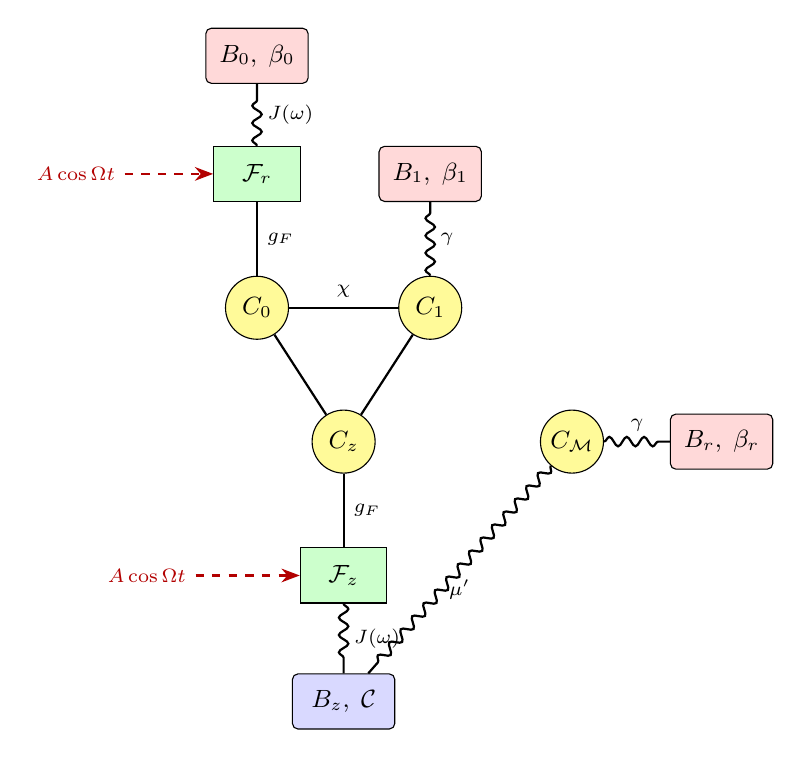
\begin{tikzpicture}[
  qubit/.style={circle, draw, fill=yellow!40, minimum size=8mm,
                inner sep=1pt, font=\small},
  bath/.style={rectangle, draw, rounded corners=2pt, fill=red!15,
               minimum width=13mm, minimum height=7mm, font=\small},
  fbath/.style={rectangle, draw, rounded corners=2pt, fill=blue!15,
                minimum width=13mm, minimum height=7mm, font=\small},
  buf/.style={rectangle, draw, fill=green!20, minimum width=11mm,
              minimum height=7mm, font=\small},
  therm/.style={decorate, decoration={snake, amplitude=.6mm,
                segment length=2.2mm, post length=1.2mm}, thick},
  coh/.style={thick},
  drv/.style={-{Stealth}, dashed, thick, red!70!black}
]
% collector qubits
\node[qubit] (C0) at (0,0)      {$C_0$};
\node[qubit] (C1) at (2.2,0)    {$C_1$};
\node[qubit] (Cz) at (1.1,-1.7) {$C_z$};
% modulator
\node[qubit] (CM) at (4.0,-1.7) {$C_\mathcal{M}$};
% buffers
\node[buf] (Fr) at (0,1.7)   {$\mathcal{F}_r$};
\node[buf] (Fz) at (1.1,-3.4){$\mathcal{F}_z$};
% baths
\node[bath]  (B0) at (0,3.2)    {$B_0,\;\beta_0$};
\node[bath]  (B1) at (2.2,1.7)  {$B_1,\;\beta_1$};
\node[bath]  (Br) at (5.9,-1.7) {$B_r,\;\beta_r$};
\node[fbath] (Bz) at (1.1,-5.0) {$B_z,\;\mathcal{C}$};
% couplings
\draw[coh] (C0) -- (C1) node[midway, above, font=\scriptsize] {$\chi$};
\draw[coh] (C0) -- (Cz);
\draw[coh] (C1) -- (Cz);
\draw[coh] (C0) -- (Fr) node[midway, right, font=\scriptsize] {$g_F$};
\draw[therm] (Fr) -- (B0) node[midway, right, font=\scriptsize]
  {$J(\omega)$};
\draw[therm] (C1) -- (B1) node[midway, right, font=\scriptsize]
  {$\gamma$};
\draw[coh] (Cz) -- (Fz) node[midway, right, font=\scriptsize] {$g_F$};
\draw[therm] (Fz) -- (Bz) node[midway, right, font=\scriptsize]
  {$J(\omega)$};
\draw[therm] (CM) -- (Br) node[midway, above, font=\scriptsize]
  {$\gamma$};
\draw[therm] (CM) -- (Bz) node[midway, below, font=\scriptsize]
  {$\mu'$};
% drives
\node[font=\scriptsize, red!70!black] (drv1) at (-2.3,1.7)
  {$A\cos\Omega t$};
\draw[drv] (drv1) -- (Fr);
\node[font=\scriptsize, red!70!black] (drv2) at (-1.4,-3.4)
  {$A\cos\Omega t$};
\draw[drv] (drv2) -- (Fz);
\end{tikzpicture}
\caption{Floquet-buffered thermodynamic NOT gate. Yellow: machine
qubits; green: driven buffer qubits with modulated gap
$\epsilon_F(t)=\epsilon_F+A\cos\Omega t$ [Eq.~\eqref{eq:bufferH}];
red: infinite baths; blue: finite output reservoir. Solid lines are
coherent (excitation-exchange) couplings, wavy lines dissipative
contacts, dashed red arrows the external drive. The input branch
$C_1\!-\!B_1$ is undressed so the logical encoding \eqref{eq:encoding}
is unchanged; the reference and output branches are filtered through
$\mathcal{F}_r$ and $\mathcal{F}_z$ respectively.}
\label{fig:buffered-architecture}
\end{figure}
 
\begin{figure}[h]
\centering
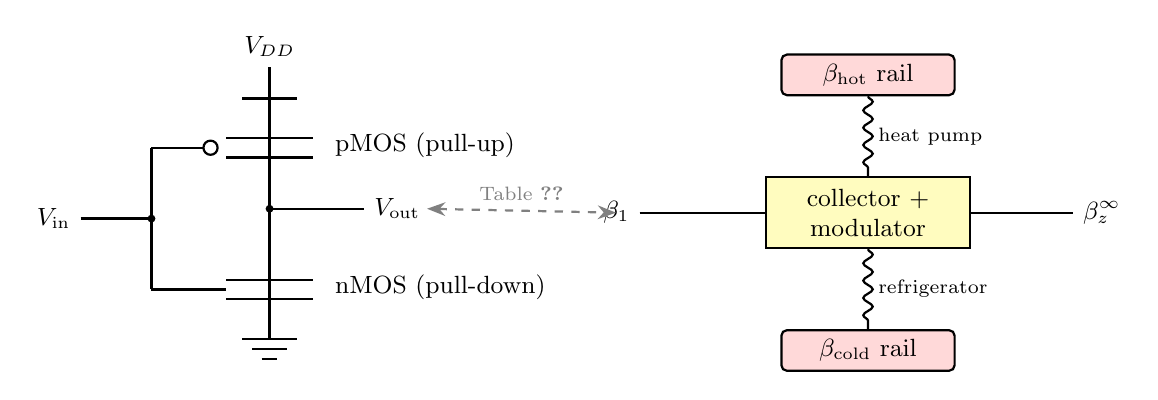
\begin{tikzpicture}[thick, font=\small]
% ---------------- CMOS inverter (left) ----------------
\begin{scope}[xshift=0cm]
  % rails
  \draw (0,4.6) node[above] {$V_{DD}$} -- (0,4.2);
  \draw (-0.35,4.2) -- (0.35,4.2);
  % pMOS: gate bar, channel bar, bubble
  \draw (0,4.2) -- (0,3.7);                       % source lead
  \draw (-0.55,3.7) -- (0.55,3.7);                % channel
  \draw (-0.55,3.45) -- (0.55,3.45);              % gate plate
  \draw[fill=white] (-0.75,3.575) circle (0.09);  % pMOS bubble
  \draw (-1.5,3.575) -- (-0.84,3.575);            % gate lead
  \draw (0,3.7) ++(0.45,0) -- ++(0,0);            % (cosmetic)
  \draw (0.45,3.7) -- (0.45,3.7);
  \draw (0,3.7) -- (0,3.2);                       % drain lead
  % nMOS
  \draw (0,2.4) -- (0,1.9);                       % drain lead
  \draw (-0.55,1.9) -- (0.55,1.9);                % channel
  \draw (-0.55,1.65) -- (0.55,1.65);              % gate plate
  \draw (-1.5,1.775) -- (-0.55,1.775);            % gate lead
  \draw (0,1.9) -- (0,1.4);                       % source lead
  % ground
  \draw (0,1.4) -- (0,1.15);
  \draw (-0.35,1.15) -- (0.35,1.15);
  \draw (-0.22,1.02) -- (0.22,1.02);
  \draw (-0.1,0.89) -- (0.1,0.89);
  % output node
  \draw (0,3.2) -- (0,2.4);
  \draw (0,2.8) -- (1.2,2.8) node[right] {$V_{\rm out}$};
  \fill (0,2.8) circle (0.05);
  % input node
  \draw (-1.5,3.575) -- (-1.5,1.775);
  \draw (-2.4,2.675) node[left] {$V_{\rm in}$} -- (-1.5,2.675);
  \fill (-1.5,2.675) circle (0.05);
  % labels
  \node[anchor=west] at (0.7,3.6) {pMOS (pull-up)};
  \node[anchor=west] at (0.7,1.8) {nMOS (pull-down)};
\end{scope}
% ---------------- neuron block (right) ----------------
\begin{scope}[xshift=7.6cm]
  \node[rectangle, draw, rounded corners=2pt, fill=red!15,
        minimum width=22mm] (hot) at (0,4.5)
        {$\beta_{\rm hot}$ rail};
  \node[rectangle, draw, rounded corners=2pt, fill=red!15,
        minimum width=22mm] (cold) at (0,1.0)
        {$\beta_{\rm cold}$ rail};
  \node[rectangle, draw, fill=yellow!25, minimum width=26mm,
        minimum height=9mm, align=center] (col) at (0,2.75)
        {collector $+$\\ modulator};
  \draw[decorate, decoration={snake, amplitude=.6mm,
        segment length=2.2mm}] (hot) -- (col)
        node[midway, right, font=\scriptsize] {heat pump};
  \draw[decorate, decoration={snake, amplitude=.6mm,
        segment length=2.2mm}] (col) -- (cold)
        node[midway, right, font=\scriptsize] {refrigerator};
  \draw (-2.9,2.75) node[left] {$\beta_1$} -- (col);
  \fill (-2.9,2.75) circle (0.0);
  \draw (col) -- (2.6,2.75) node[right] {$\beta_z^\infty$};
\end{scope}
% mapping arrows
\draw[{Stealth}-{Stealth}, dashed, gray]
  (2.0,2.8) -- (4.4,2.75)
  node[midway, above, font=\scriptsize, text=gray]
  {Table~\ref{tab:cmos-dictionary}};
\end{tikzpicture}
\caption{Structural correspondence. Left: static CMOS inverter; the
complementary pair pulls the output to one rail and cuts off the path
to the other. Right: the neuron's two thermodynamic regimes play the
roles of the pull-up/pull-down networks, with the modulator providing
rail restoration; unlike CMOS, no regime is ever fully ``cut off'' ---
the NESS dissipates continuously, which the gated output buffer
$\mathcal{F}_z$ mitigates at the cost of clock work
(Sec.~\ref{sec:output-buffer}).}
\label{fig:cmos-correspondence}
\end{figure}
 































\newpage



\part{Abhishek: Periodically Driven Open‑System Logic Gates}
\label{part:abhishek}

\section{Introduction}
\subsection{What is thermodynamic computing?}
Thermodynamic computing \cite{Conte2019} proposes that the natural relaxation of a physical system coupled to heat baths can be harnessed to perform computation. In the quantum regime, autonomous thermal machines composed of a few interacting qubits can act as ``thermodynamic neurons'': logical inputs are encoded in the temperatures of finite‑size heat baths, and the logical output is read from the temperature of an auxiliary output bath once the system has settled into a nonequilibrium steady state (NESS) \cite{LipkaBartosik2024, Meier2025}. The key appeal is that such devices operate without an external clock: computation is driven entirely by the flow of heat from hot to cold reservoirs.

\subsection{Why add periodic driving?}
All existing quantum thermodynamic neurons are \emph{autonomous}, i.e., their Hamiltonians are time‑independent. In this note we ask a natural question: can one improve the speed or accuracy of a thermodynamic neuron by adding a periodic driving field? This is a form of \emph{Floquet engineering}: a periodically driven auxiliary system (the \emph{Floquet buffer}) is inserted between the logical qubits and the physical baths. The buffer acts as a tunable effective environment whose spectral density can be shaped by the drive.

The price is twofold. First, the device is no longer autonomous; it requires a classical clock to maintain the drive and to read out the result stroboscopically. Second, an external work input is needed to power the drive. Nevertheless, the resulting architecture---a \emph{periodically driven dissipative logic gate}---is an interesting candidate for low‑energy computation.

\subsection{Scope and structure of this note}
This note is written as a self‑contained pedagogical resource for a collaborative project involving a theoretical physicist, a mathematician working on tensor networks, and an MSc student with a background in engineering and coding. We assume familiarity with basic quantum mechanics (Hilbert spaces, operators, partial trace, von Neumann equation) and statistical mechanics (canonical ensemble, partition function). All more advanced concepts (GKSL equation, Floquet theory, chain mapping of baths, matrix‑product states) are reviewed in the main text or in the appendices.

The note is organised as follows.
\begin{itemize}
    \item Section~\ref{sec:background} provides concise reviews of the GKSL master equation, Floquet theory, the chain representation of bosonic baths, matrix‑product states (MPS), and the trace distance as a distinguishability measure.
    \item Section~\ref{sec:architecture} describes the Floquet‑buffer architecture in detail.
    \item Section~\ref{sec:weak} states and proves a theorem (Proposition~\ref{prop:periodic}) that in a certain weak‑coupling limit the logical qubits obey a time‑periodic GKSL equation.
    \item Section~\ref{sec:nonMarkovian} explains how to go beyond weak coupling using chain mapping and MPS, and how to extract energy currents and work without exponentially large bond dimensions.
    \item Section~\ref{sec:conjecture} proposes a conjectured work–distinguishability tradeoff.
    \item Section~\ref{sec:numerics} outlines a staged numerical programme.
    \item The appendices contain additional technical details.
\end{itemize}

\section{Background material}\label{sec:background}
Here we collect, in a deliberately compact form, the mathematical tools that are essential for the rest of the note. The reader may skip this section on first reading and return as needed.

\subsection{GKSL (Lindblad) master equation}\label{sec:GKSL}
A Markovian open quantum system is described by a density matrix $\rho$ evolving under the GKSL (Gorini‑Kossakowski‑Sudarshan‑Lindblad) equation:
\begin{equation}\label{eq:GKSL_general}
\dot\rho = -\ii[H,\rho] + \sum_k \gamma_k \Big( L_k \rho L_k^\dagger - \tfrac12 \{ L_k^\dagger L_k, \rho \} \Big),
\end{equation}
where $H$ is the effective system Hamiltonian, $L_k$ are jump operators, and $\gamma_k\ge0$ are positive rates. The generator is trace‑preserving and completely positive. If the rates satisfy local detailed balance with respect to a heat bath at inverse temperature $\beta$, the system relaxes to a Gibbs state $\rho_\beta\propto\ee^{-\beta H}$ (when there is only one bath) or to a NESS when several baths are present.

\subsection{Floquet theory and Floquet‑Lindblad equation}\label{sec:Floquet}
A periodically driven system has a Hamiltonian $H(t)=H(t+T)$ with $T=2\pi/\Omega$. The time‑evolution operator can be written in terms of Floquet modes $\ket{\phi_n(t)}$ and quasi‑energies $\epsilon_n$:
\begin{equation}
U(t) = \sum_n \ee^{-\ii \epsilon_n t} \ket{\phi_n(t)}\bra{\phi_n(0)},
\end{equation}
where $\ket{\phi_n(t+T)}=\ket{\phi_n(t)}$ and $\epsilon_n\in[-\Omega/2,\Omega/2)$.

When the system is open and weakly coupled to one or more baths, a Floquet‑Lindblad equation can be derived \cite{Kurizki2015, Brandner2016}. The generator becomes time‑periodic:
\begin{equation}
\dot\rho(t) = \mathcal{L}(t)\rho(t),\qquad \mathcal{L}(t+T)=\mathcal{L}(t).
\end{equation}
The jump operators are expressed in the Floquet basis, and the rates depend on the Fourier components of the bath correlation functions at frequencies shifted by multiples of $\Omega$. A crucial feature is the appearance of sidebands: transitions can occur at energies $\epsilon_m-\epsilon_n + q\Omega$, $q\in\bbZ$, which allows the system to absorb or emit quanta of the drive while exchanging energy with the baths.

\subsection{Chain mapping of bosonic baths}\label{sec:chain}
A heat bath is usually modelled as a collection of independent harmonic oscillators:
\begin{equation}
H_B = \int_0^\infty \d\omega\, \omega\, a_\omega^\dagger a_\omega,
\end{equation}
coupled to the system by $H_{SB} = A\otimes \int \d\omega\, \sqrt{J(\omega)}(a_\omega+a_\omega^\dagger)$, where $J(\omega)$ is the spectral density. For numerical purposes it is convenient to map this continuum model to a semi‑infinite one‑dimensional chain with nearest‑neighbour hopping \cite{Chin2010, Prior2010}. The transformation uses a sequence of orthogonal polynomials (e.g., Lanczos or Chebyshev) determined by $J(\omega)$. After the mapping, the Hamiltonian becomes
\begin{equation}\label{eq:chainH}
H_{\text{chain}} = \sum_{k=1}^\infty \omega_k a_k^\dagger a_k + \sum_{k=1}^\infty t_k (a_k^\dagger a_{k+1} + a_{k+1}^\dagger a_k),
\end{equation}
where $a_k$ ($k\ge1$) are new bosonic operators, and the system couples only to the first site: $H_{SB} \propto A\otimes (a_1 + a_1^\dagger)$. The parameters $\omega_k$ and $t_k$ are determined recursively from the spectral density. For an Ohmic bath $J(\omega)\propto\omega$ with a suitable cutoff, the coefficients $t_k$ decay rapidly with $k$, so that a truncation to a finite chain of length $N$ (typically $N\sim 100-200$) gives converged results for the reduced system dynamics.

\subsection{Matrix‑product states (MPS) and the TDVP}\label{sec:MPS}
A one‑dimensional quantum lattice system (such as the chain‑mapped bath) can be efficiently represented by a matrix‑product state:
\begin{equation}
\ket{\psi} = \sum_{\{s_i\}} C^{s_1} A^{s_2} \cdots A^{s_N} \ket{s_1 s_2 \dots s_N},
\end{equation}
where $C$ and $A^{s_i}$ are matrices, and the bond dimension $\chi$ controls the amount of entanglement that can be captured. The time‑dependent variational principle (TDVP) or Trotter‑Suzuki decompositions allow one to evolve the MPS in real time under a Hamiltonian $H(t)$. The computational cost scales as $O(N\chi^3 d^2)$ per time step, where $d$ is the local Hilbert space dimension.

For the chain‑mapped bath at moderate temperature, the entanglement entropy between the system and the first few chain sites saturates at a finite value. Consequently, the required bond dimension $\chi$ does not grow with the chain length $N$; values of $\chi\approx 30$–$50$ are typical for converged simulations.

\subsection{Trace distance as a distinguishability measure}\label{sec:trace}
The trace distance between two density matrices $\rho$ and $\sigma$ is
\begin{equation}
D(\rho,\sigma) = \tfrac12 \norm{\rho-\sigma}_1,
\end{equation}
where $\norm{A}_1=\Tr\sqrt{A^\dagger A}$. It satisfies $0\le D(\rho,\sigma)\le 1$ and is a metric on the space of states. Operationally, $D(\rho,\sigma)$ is equal to the maximum success probability of distinguishing $\rho$ from $\sigma$ with a single measurement. We will use it to quantify the logical distinguishability: for a binary logic gate, the two possible output states $\rho_{\text{out}}^{(0)}$ and $\rho_{\text{out}}^{(1)}$ are perfectly distinguishable when $D=1$, and completely indistinguishable when $D=0$.

\section{Architecture of the Floquet‑buffered logic gate}\label{sec:architecture}
The physical device is sketched in Fig.~\ref{fig:schematic}. It consists of:
\begin{itemize}
    \item \textbf{Logical qubits} $\calS$, described by a time‑independent Hamiltonian $H_S$. For concreteness, in the numerical programme we will use three qubits forming a NOR gate as in \cite{LipkaBartosik2024}.
    \item \textbf{Floquet buffer} $\calB_F$, a finite quantum system with a time‑periodic Hamiltonian $H_{\text{buf}}(t)=H_{\text{buf}}(t+T)$, $T=2\pi/\Omega$. The buffer could be, for example, a harmonic oscillator with a modulated frequency or a driven two‑level system.
    \item \textbf{System‑buffer coupling} $H_{S\text{buf}}$, assumed time‑independent and, for the weak‑coupling theorem, weak.
    \item \textbf{Thermal baths}, each at a different temperature $T_\alpha$, coupled only to the buffer via $H_{\text{buf},B_\alpha}$.
\end{itemize}

The logical input is encoded in the temperatures $\{T_\alpha\}$ of the baths, exactly as in the autonomous thermodynamic neuron. The output, however, is not read from an auxiliary bath; instead, we measure an observable of the output qubit stroboscopically at times $t_n=nT$, after a periodic steady state has been reached. This is a deliberate departure from strict autonomy: the device requires an external clock to synchronise the drive and the readout.

The reasons for this choice are twofold. First, in the autonomous model the output bath temperature depends on the qubit‑bath coupling, which is absent in our architecture (the qubits couple only to the buffer). Second, stroboscopic readout is natural in Floquet systems and is used in many quantum computing platforms.

Because we accept a clock, the thermodynamics of the device is that of a periodically driven open system. The relevant energetic quantities are the cycle‑averaged work $\overline{W}$ provided by the drive and the cycle‑averaged heat currents $\overline{J}_\alpha$ into the baths.

\begin{figure}[h]
\centering
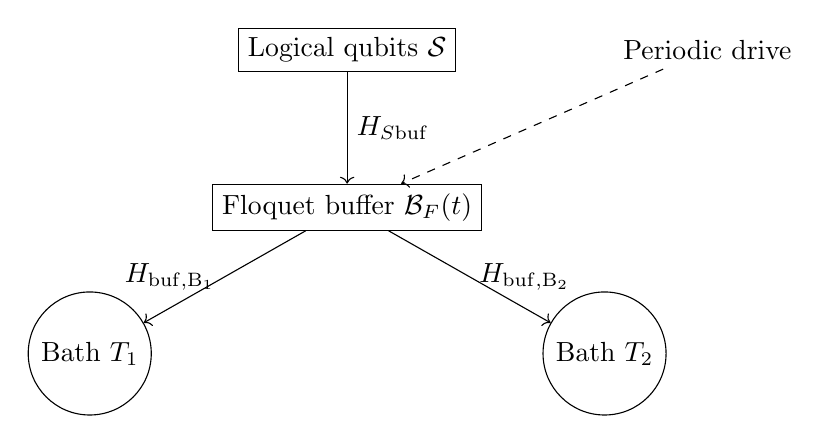
\begin{tikzpicture}[node distance=2cm]
\node[draw, rectangle] (qubits) {Logical qubits $\calS$};
\node[draw, rectangle, below of=qubits] (buffer) {Floquet buffer $\calB_F(t)$};
\node[draw, circle, below left=1cm and 1cm of buffer] (bath1) {Bath $T_1$};
\node[draw, circle, below right=1cm and 1cm of buffer] (bath2) {Bath $T_2$};
\draw[->] (qubits) -- (buffer) node[midway, right] {$H_{S\rm buf}$};
\draw[->] (buffer) -- (bath1) node[midway, left] {$H_{\rm buf, B_1}$};
\draw[->] (buffer) -- (bath2) node[midway, right] {$H_{\rm buf, B_2}$};
\node[right=2cm of qubits] (drive) {Periodic drive};
\draw[->,dashed] (drive) -- (buffer);
\end{tikzpicture}
\caption{Periodically driven logic gate with Floquet buffer. The logical qubits interact only with the driven buffer; the buffer couples to thermal reservoirs. The device is not fully autonomous: a classical clock synchronises the drive and the stroboscopic readout.}
\label{fig:schematic}
\end{figure}

\section{Weak‑coupling regime: periodic GKSL generator}\label{sec:weak}
Under certain idealised conditions, one can eliminate the buffer and the baths and obtain a closed description of the logical qubits alone.

\subsection{Assumptions}
We impose:
\begin{enumerate}[label=(A\arabic*),leftmargin=*]
    \item \textbf{Weak buffer‑bath coupling.} The interactions $H_{\text{buf},B_\alpha}$ are sufficiently weak that the buffer, when decoupled from $\calS$, relaxes to a unique periodic steady state $\rho_{\text{buf},ss}(t)$ under the Floquet‑Lindblad equation. The generator of this buffer‑only dynamics is $\mathcal{L}_{\text{buf}}(t)$.
    \item \textbf{Exponential decay of buffer correlations.} In that periodic steady state, the two‑time correlation functions $\langle B_i(t)B_j(t-\tau)\rangle$ decay to zero on a characteristic time scale $\tau_c$. More precisely, there exists $\tau_c$ such that $|C_{ij}(t,\tau)|<\varepsilon$ for $\tau>\tau_c$ for any chosen tolerance $\varepsilon$.
    \item \textbf{Weak system‑buffer coupling and time‑scale separation.} The coupling $H_{S\text{buf}}$ is much weaker than the buffer’s internal relaxation scale, and the logical qubits evolve slowly compared to $\tau_c$. This allows us to apply the Born–Markov approximation.
    \item \textbf{Secular approximation.} The Bohr frequencies (transition frequencies) of $H_S$ are non‑degenerate and well separated compared to the relaxation rates induced by the buffer.
\end{enumerate}

\subsection{Periodic GKSL generator}
\begin{proposition}\label{prop:periodic}
Under Assumptions (A1)–(A4), there exists a time‑periodic generator $\mathcal{L}_{\text{eff}}(t)$ of the form
\begin{equation}
\mathcal{L}_{\text{eff}}(t)\rho = -\ii[H_S + H_{LS}(t), \rho] + \sum_k \Gamma_k(t) \Big( L_k(t) \rho L_k^\dagger(t) - \tfrac12\{ L_k^\dagger(t)L_k(t),\rho \} \Big),
\end{equation}
with $\mathcal{L}_{\text{eff}}(t+T)=\mathcal{L}_{\text{eff}}(t)$, such that the reduced state of the logical qubits obeys
\begin{equation}\label{eq:periodic_dyn}
\dot\rho_S(t) = \mathcal{L}_{\text{eff}}(t)\rho_S(t).
\end{equation}
The jump operators $L_k(t)$ and rates $\Gamma_k(t)$ are obtained from the Fourier transforms of the buffer correlation functions evaluated at the Bohr frequencies of $H_S$, including sideband shifts by multiples of $\Omega$.
\end{proposition}

\paragraph{Proof sketch.}
The derivation follows the standard Floquet–Born–Markov approach \cite{Kurizki2015}. One starts from the Nakajima–Zwanzig equation with the buffer acting as a structured environment. The memory kernel is of second order in $H_{S\text{buf}}$. Because of (A2) the kernel decays on the time scale $\tau_c$, and because of (A3) the system density matrix changes slowly on that scale; we can therefore make the Markov approximation and replace the memory integral by a time‑local superoperator. The time dependence of this superoperator is inherited from the periodic buffer steady state. The secular approximation (A4) diagonalises the dynamics in the eigenbasis of $H_S$, yielding the GKSL form with time‑periodic coefficients.

\paragraph{Practical limitations.}
The assumptions are strong. In particular, the weak‑coupling condition (A3) may be hard to satisfy simultaneously with (A1) because weak buffer‑bath coupling implies a long buffer correlation time, whereas a Markovian elimination requires the buffer correlations to decay fast \emph{relative to the qubit dynamics}. Therefore Proposition~\ref{prop:periodic} should be seen as identifying a parameter window in which a simple theoretical description exists, not as a statement about generic parameters.

A second issue is the dynamic Lamb shift. The Floquet buffer will induce time‑dependent shifts $H_{LS}(t)$ in the qubit energy levels. The autonomous thermodynamic NOT gate relies on a precise resonance condition $\omega_W = \omega_X + \omega_Y$ among three qubit frequencies. The Floquet‑induced Lamb shift will generically detune this resonance and destroy the logical operation. To mitigate this, we must actively adjust the bare qubit frequencies as functions of the drive amplitude, a procedure that is realistic in circuit‑QED architectures but constitutes an additional control overhead.

For all these reasons, the main numerical programme of this project targets the regime \emph{outside} the validity of Proposition~\ref{prop:periodic}, where no simple Lindbladian exists. Nevertheless, the weak‑coupling analysis is a useful conceptual starting point.

\section{Non‑Markovian regime: chain mapping and MPS}\label{sec:nonMarkovian}
To treat arbitrary coupling strengths and memory effects, we simulate the full system‑buffer‑baths compound as a closed many‑body quantum system. We employ two established techniques: chain mapping of the baths (Sec.~\ref{sec:chain}) and matrix‑product state evolution (Sec.~\ref{sec:MPS}).

\subsection{Chain‑mapped Hamiltonian}
Starting from the original bath model with a continuum of harmonic oscillators and a given spectral density $J(\omega)$, we apply a unitary transformation (Lanczos or orthogonal‑polynomial mapping) that yields the chain Hamiltonian \eqref{eq:chainH}. The total Hamiltonian in the chain picture is
\begin{equation}\label{eq:total_chain}
\begin{aligned}
H_{\text{tot}}(t) &= H_S \;+\; H_{\text{buf}}(t) \;+\; H_{S\text{buf}} \\
&\quad + \sum_{\alpha} \Big[ \sum_{k=1}^{N_\alpha} \omega_{\alpha k} a_{\alpha k}^\dagger a_{\alpha k}
   + \sum_{k=1}^{N_\alpha-1} t_{\alpha k} (a_{\alpha k}^\dagger a_{\alpha,k+1} + \text{h.c.}) \Big] \\
&\quad + \sum_{\alpha} V_{\text{buf},\alpha} \otimes (a_{\alpha 1} + a_{\alpha 1}^\dagger).
\end{aligned}
\end{equation}
Here $N_\alpha$ is the chain length for bath $\alpha$ (chosen large enough to suppress finite‑size effects), and $V_{\text{buf},\alpha}$ is a buffer operator determined by the original buffer‑bath coupling.

This Hamiltonian describes a one‑dimensional lattice system. The logical qubits sit at the leftmost end, the buffer is next, and each bath forms a separate chain. The only interaction between qubits and baths is mediated by the buffer: the qubits couple to the buffer, and the buffer couples to the first site of each chain.

\subsection{Energy current and work}
Because the chain Hamiltonian is a closed system, thermodynamic observables can be defined exactly from the Heisenberg equations of motion.

The energy current from the logical qubits into the buffer is the time derivative of the qubit energy minus the contribution that would occur without the coupling:
\begin{equation}\label{eq:current_def}
J_{S\to\text{buf}}(t) = \ii\big\langle [H_S,\, H_{S\text{buf}}] \big\rangle.
\end{equation}
Here $\langle\cdot\rangle = \Tr(\rho_{\text{tot}}(t)\cdot)$, with $\rho_{\text{tot}}$ the state of the full chain. Because $H_S$ acts only on the qubits and $H_{S\text{buf}}$ acts on qubits and buffer, the commutator is a local operator with support on the qubits and the buffer alone. Its expectation value can therefore be computed directly from the MPS representation of the state without needing to reconstruct the full bath density matrix.

The power injected by the periodic drive is
\begin{equation}\label{eq:power_def}
P_{\text{drive}}(t) = \Big\langle \frac{\partial H_{\text{buf}}(t)}{\partial t} \Big\rangle.
\end{equation}
This is also a local observable (it acts only on the buffer). The cycle‑averaged work is
\begin{equation}
\overline{W} = \frac1T \int_0^T P_{\text{drive}}(t)\,\d t.
\end{equation}

The heat dumped into bath $\alpha$ can be obtained from the energy current flowing from the buffer into the first site of chain $\alpha$, using the buffer‑chain coupling. This current is again a local observable.

\subsection{Bond‑dimension control}
A crucial practical question is whether the MPS simulation remains tractable. For a one‑dimensional chain with nearest‑neighbour couplings, the entanglement entropy of the state follows an area law: for a gapped system it saturates to a constant; for a critical (gapless) system it grows logarithmically with the chain length. The chain‑mapped bath is gapless (the site frequencies $\omega_k$ extend to zero), but the coupling $t_k$ decays rapidly with $k$, so that only the first few tens of sites are strongly entangled with the system.

In practice, for an Ohmic spectral density with a high‑frequency cutoff and for temperatures $k_B T$ above the smallest energy scale of the chain, the bond dimension required for convergence is $\chi \approx 30$–$50$. This value does \emph{not} increase when the chain length $N$ is increased beyond the point where the first few sites have captured the relevant physics. The computational cost per time step then scales as $O(N\chi^3 d^2)$, where $d$ is the local Hilbert space dimension. For a truncated Fock space with $d=10$–$20$, this is manageable for the single‑qubit buffer prototype (Phase~3 of the numerical programme) and, with tree‑tensor‑network (TTN) enhancements, for the three‑qubit gate (Phase~4).

\section{Conjectured work–distinguishability tradeoff}\label{sec:conjecture}
In the autonomous thermodynamic neuron, logical distinguishability is intrinsically linked to the temperature difference between the baths; increasing the distinguishability requires a larger temperature gradient, which implies larger entropy production. In our driven setting, we expect a similar tradeoff: improving the logical distinguishability beyond the undriven baseline should require a positive amount of work per cycle.

Formally, let
\begin{equation}
P_{\text{dist}} = \tfrac12 \norm{ \rho_{\text{out}}^{(0)} - \rho_{\text{out}}^{(1)} }_1
\end{equation}
be the trace‑distance distinguishability of the output qubit states corresponding to the two logical inputs. Let $P_{\text{dist}}^{(0)}$ be this quantity when the buffer is undriven (i.e., the baseline autonomous gate, but with the same qubit readout), and let $\overline{W}$ be the cycle‑averaged work when the buffer is driven.

\begin{conjecture}[Work–distinguishability tradeoff]\label{conj:tradeoff}
There exists a monotonically increasing function $f$ with $f(P_{\text{dist}}^{(0)})=0$ such that
\begin{equation}
\overline{W} \ge f(P_{\text{dist}}).
\end{equation}
In particular, any enhancement $P_{\text{dist}} > P_{\text{dist}}^{(0)}$ requires $\overline{W}>0$.
\end{conjecture}

This conjecture is motivated by known thermodynamic uncertainty relations (TURs) and speed‑limit inequalities, which bound the precision of a process in terms of the entropy production or work. The precise functional form of $f$ and its dependence on the bath temperatures are open questions that the numerical programme will explore.

\section{Numerical programme}\label{sec:numerics}
We propose a staged numerical investigation, designed to proceed from controlled to more challenging regimes.

\paragraph{Phase 1: Undriven baseline.}
Reproduce the autonomous NOT gate of \cite{LipkaBartosik2024} using QuTiP. However, instead of reading the output from a bath temperature, we read it from the reduced state of a designated output qubit. This gives us the undriven distinguishability $P_{\text{dist}}^{(0)}$ and the baseline steady‑state heat currents.

\paragraph{Phase 2: Weak‑coupling Floquet buffer (QuTiP).}
Implement a single qubit coupled to a driven harmonic oscillator (the buffer), which is weakly coupled to two Ohmic baths. Use QuTiP’s Floquet‑Lindblad module to numerically verify Proposition~\ref{prop:periodic}. Explore how $P_{\text{dist}}$ and $\overline{W}$ depend on drive amplitude and frequency. Check whether the conjecture holds in this regime.

\paragraph{Phase 3: MPS chain simulation (single qubit).}
Build the chain‑mapped model of one qubit, one driven buffer, and two thermal chains using ITensor or MPSDynamics.jl. Initialise the chains in thermal states (via thermofield purification). Evolve in time until the periodic steady state is reached, then compute the energy current \eqref{eq:current_def}, the drive power \eqref{eq:power_def}, and the output qubit distinguishability. Investigate parameter regimes where the weak‑coupling assumptions fail, and test the conjecture beyond weak coupling.

\paragraph{Phase 4: Three‑qubit NOR gate.}
Extend the chain mapping to the full three‑qubit NOR gate with a single Floquet buffer. Here the bond dimension may grow; if it becomes prohibitive, we will use tree tensor networks (TTNs) or systematic truncation of the least‑coupled chain sites. The goal is to produce a phase diagram of $P_{\text{dist}}$ as a function of drive amplitude and frequency, and to test the conjecture for a practical logic gate.

All code and data will be made publicly available to facilitate reproducibility.

\section{Conclusion}
We have presented a self‑contained, pedagogical introduction to the Floquet‑buffer architecture for periodically driven logic gates. The note reviews the necessary technical background, states a rigorous theorem in the weak‑coupling limit, explains how to treat the non‑Markovian regime with chain‑mapped MPS, and formulates a clear conjecture to be tested numerically. The project is designed to utilise the complementary strengths of the collaboration: the physicist’s formal analysis, the mathematician’s tensor‑network expertise, and the student’s numerical skills. This note is the definitive starting point for the work.

\begin{appendices}
\section{Derivation of the GKSL equation from a microscopic model}
For completeness we sketch the derivation of the GKSL equation \eqref{eq:GKSL_general} from a system‑bath Hamiltonian. Consider a system $S$ coupled to a bath $B$ via $H_{SB}= \sum_i S_i\otimes B_i$. In the Born–Markov approximation, after tracing out the bath, one obtains the Redfield equation. The additional secular (rotating‑wave) approximation diagonalises the dynamics in the eigenbasis of $H_S$ and ensures complete positivity. The resulting jump operators are the eigenoperators $A(\omega)$ of the system Hamiltonian, with rates $\gamma(\omega)= \int e^{i\omega t}\langle B^\dagger(t)B(0)\rangle dt$. The detailed balance condition $\gamma(-\omega)=e^{-\beta\omega}\gamma(\omega)$ follows from the KMS condition of the bath. See \cite{Breuer2002} for a textbook treatment.

\section{Chain mapping: recurrence relations}
Given a spectral density $J(\omega)$, the chain mapping is constructed by orthogonalising the polynomials in $\omega$ with respect to the measure $J(\omega)d\omega$. The recurrence coefficients $\omega_k$ and $t_k$ are obtained from the continued fraction expansion of the bath correlation function. For the common case of an Ohmic bath with exponential cutoff, $J(\omega)= \eta\omega e^{-\omega/\omega_c}$, the coefficients can be computed analytically or numerically using the Lanczos algorithm \cite{Chin2010}.

\section{MPS representation of a thermal state}
To initialise the chain in a thermal state at temperature $T$, one uses the thermofield (purification) approach. Each physical bosonic site is doubled into an ancilla site, and the initial state is the vacuum for a set of Bogoliubov‑transformed modes. The resulting MPS bond dimension is directly related to the effective temperature; for moderate $T$, it remains small.

\section{Energy current operator: explicit form}
Equation \eqref{eq:current_def} follows from the Heisenberg equation for $H_S$:
\begin{equation}
\frac{d H_S}{dt} = \ii[ H_{\text{tot}}, H_S ] = \ii[ H_S, H_{S\text{buf}} ] + \ii[ H_S, H_S ] = \ii[ H_S, H_{S\text{buf}} ].
\end{equation}
The term $[H_S, H_S]=0$, and $H_S$ commutes with all bath and buffer‑bath Hamiltonians because it acts on a different tensor factor. Hence the energy change of the qubits is solely due to the qubit‑buffer interaction. Taking the expectation value gives the current.
\end{appendices}

\begin{thebibliography}{99}
\bibitem{Conte2019} T.~Conte et al., “Thermodynamic Computing,” arXiv:1911.01968 (2019).
\bibitem{LipkaBartosik2024} P.~Lipka-Bartosik, M.~Perarnau-Llobet, and N.~Brunner, “Thermodynamic computing via autonomous quantum thermal machines,” Sci.\ Adv.\ \textbf{10}, eadm8792 (2024).
\bibitem{Meier2025} F.~Meier, S.~Huber, P.~Erker, and A.~Xuereb, “Autonomous Quantum Processing Unit,” arXiv:2501.15615 (2025).
\bibitem{Kurizki2015} D.~Gelbwaser-Klimovsky, W.~Niedenzu, and G.~Kurizki, “Thermodynamics of quantum systems under dynamical control,” Adv.\ At.\ Mol.\ Opt.\ Phys.\ \textbf{64}, 329 (2015).
\bibitem{Brandner2016} K.~Brandner and U.~Seifert, “Periodic thermodynamics of open quantum systems,” Phys.\ Rev.\ E \textbf{93}, 062134 (2016).
\bibitem{Chin2010} A.~W.~Chin, \'{A}.~Rivas, S.~F.~Huelga, and M.~B.~Plenio, “Exact mapping between system‑reservoir quantum models and semi‑infinite discrete chains,” J.\ Math.\ Phys.\ \textbf{51}, 092109 (2010).
\bibitem{Prior2010} J.~Prior, A.~W.~Chin, S.~F.~Huelga, and M.~B.~Plenio, “Efficient simulation of strong system‑environment interactions,” Phys.\ Rev.\ Lett.\ \textbf{105}, 050404 (2010).
\bibitem{Wolpert2022} D.~H.~Wolpert, “Stochastic thermodynamics of computation,” J.\ Stat.\ Phys.\ \textbf{187}, 10 (2022).
\bibitem{Breuer2002} H.-P.~Breuer and F.~Petruccione, \textit{The Theory of Open Quantum Systems}, Oxford University Press (2002).
\bibitem{TienGordon1963} P.~K.~Tien and J.~P.~Gordon, ``Multiphoton Process Observed in the Interaction of Microwave Fields with the Tunneling between Superconductor Films,'' Phys.\ Rev.\ \textbf{129}, 647 (1963).
\bibitem{Grifoni1998} M.~Grifoni and P.~H\"anggi, ``Driven quantum tunneling,'' Phys.\ Rep.\ \textbf{304}, 229 (1998).
\bibitem{OQuPy} G.~E.~Fux, D.~Kilda, B.~W.~Lovett, and J.~Keeling, “OQuPy: A Python package to efficiently simulate non‑Markovian open quantum systems,” J.\ Chem.\ Phys.\ \textbf{161}, 124108 (2024).

\bibitem{QuTiP}
J. R. Johansson, P. D. Nation, and F. Nori,
``QuTiP: An open-source Python framework for the dynamics of open quantum systems,''
\textit{Computer Physics Communications},
vol. 183, no. 8, pp. 1760--1772, Aug. 2012.
DOI: \url{https://doi.org/10.1016/j.cpc.2012.02.021}.

\end{thebibliography}

\end{document}


